\PassOptionsToPackage{table}{xcolor}
\documentclass[11pt,a4paper]{article}

% ==============================================================================
% PACKAGES & GEOMETRY
% ==============================================================================
\usepackage[a4paper,margin=1.8cm,headheight=26pt,top=2.2cm,bottom=2.0cm]{geometry}
\usepackage{fontspec}
\usepackage{amsmath,amssymb}
\usepackage{enumitem}
\setlist{nosep,leftmargin=1.4em,topsep=2pt,itemsep=2pt}
\usepackage{booktabs}
\usepackage{colortbl}
\usepackage{tabularx}
\usepackage{array}
\usepackage{tikz}
\usetikzlibrary{shapes,backgrounds,arrows.meta,positioning,calc}
\usepackage{xcolor}
\usepackage[most]{tcolorbox}
\tcbuselibrary{skins,breakable}
\usepackage{fancyhdr}
\usepackage{titlesec}
\usepackage{titletoc}

% Styled Table of Contents
\titlecontents{section}[0pt]
  {\addvspace{7pt}\bfseries\color{navy}}
  {\contentslabel[\thecontentslabel]{1.8em}}
  {}
  {\titlerule*[0.5pc]{\color{gray!60}.}\bfseries\color{teal}\contentspage}

\titlecontents{subsection}[2.4em]
  {\addvspace{1.5pt}\normalfont\small\color{darkslate}}
  {\contentslabel[\thecontentslabel]{2.2em}}
  {}
  {\titlerule*[0.5pc]{\color{gray!35}.}\color{teal!80!black}\contentspage}

\usepackage[colorlinks=true,linkcolor=teal,urlcolor=teal,citecolor=navy]{hyperref}

% ==============================================================================
% COLOR PALETTE (Navy / Teal / Gold / Coral)
% ==============================================================================
\definecolor{navy}{HTML}{0B2545}
\definecolor{teal}{HTML}{147D75}
\definecolor{gold}{HTML}{C9A227}
\definecolor{lightteal}{HTML}{E7F3F2}
\definecolor{lightgold}{HTML}{FBF3DD}
\definecolor{coral}{HTML}{C0392B}
\definecolor{lightcoral}{HTML}{FDEDEC}
\definecolor{darkslate}{HTML}{1E293B}

% ==============================================================================
% TCOLORBOX ENVIRONMENTS
% ==============================================================================
\newtcolorbox{defbox}[1][Definition]{
  colback=lightteal, colframe=teal, coltitle=white,
  fonttitle=\bfseries\small, colbacktitle=teal,
  title={#1},
  breakable, boxrule=0.8pt, arc=3pt,
  left=8pt, right=8pt, top=6pt, bottom=6pt,
  before skip=6pt, after skip=6pt
}

\newtcolorbox{examplebox}[1][Concrete Example]{
  colback=lightgold, colframe=gold, coltitle=navy,
  fonttitle=\bfseries\small, colbacktitle=lightgold,
  title={#1},
  breakable, boxrule=0.8pt, arc=3pt,
  left=8pt, right=8pt, top=6pt, bottom=6pt,
  before skip=6pt, after skip=6pt
}

\newtcolorbox{theorembox}[1][Proof \& Derivation]{
  colback=white, colframe=navy, coltitle=white,
  fonttitle=\bfseries\small, colbacktitle=navy,
  title={#1},
  breakable, boxrule=1pt, arc=3pt,
  left=8pt, right=8pt, top=6pt, bottom=6pt,
  before skip=6pt, after skip=6pt
}

\newtcolorbox{warningbox}[1][Beginner Trap \& Watch Out!]{
  colback=lightcoral, colframe=coral, coltitle=white,
  fonttitle=\bfseries\small, colbacktitle=coral,
  title={#1},
  breakable, boxrule=0.9pt, arc=3pt,
  left=8pt, right=8pt, top=6pt, bottom=6pt,
  before skip=6pt, after skip=6pt
}

\newtcolorbox{notebox}[1][Key Takeaway / Summary]{
  colback=navy!5, colframe=navy!70, coltitle=white,
  fonttitle=\bfseries\small, colbacktitle=navy!70,
  title={#1},
  breakable, boxrule=0.7pt, arc=3pt,
  left=8pt, right=8pt, top=6pt, bottom=6pt,
  before skip=6pt, after skip=6pt
}

\newtcolorbox{exambox}[1]{
  colback=white, colbacklower=teal!6, colframe=navy!90, coltitle=white,
  fonttitle=\bfseries\small, colbacktitle=navy!90,
  title={#1},
  breakable, boxrule=0.9pt, arc=3pt,
  left=8pt, right=8pt, top=6pt, bottom=7pt,
  before skip=6pt, after skip=6pt,
  lower separated=true, borderline horizontal={0.6pt}{0pt}{gold}
}
% Q/A label helpers for consistent, distinguishable exam boxes
\newcommand{\Qlabel}{\textbf{\color{navy}\footnotesize\MakeUppercase{Question}}\par\smallskip}
\newcommand{\Alabel}{\textbf{\color{teal}\footnotesize\MakeUppercase{Answer}}\par\smallskip}

% ==============================================================================
% HEADER & FOOTER
% ==============================================================================
\pagestyle{fancy}
\fancyhf{}
\renewcommand{\headrulewidth}{0.8pt}
\renewcommand{\headrule}{\hbox to\headwidth{\color{teal}\leaders\hrule height \headrulewidth\hfill}}
\renewcommand{\footrulewidth}{0.4pt}
\fancyhead[L]{\small\bfseries\color{navy} CSE 1143: Discrete Mathematics}
\fancyhead[R]{\small\bfseries\color{teal} Sets \& Relations}
\fancyfoot[L]{\footnotesize\color{gray} Suleman Ahmed Shuvo}
\fancyfoot[R]{\footnotesize\bfseries\color{navy} Page \thepage}

% ==============================================================================
% SECTION TITLES
% ==============================================================================
\titleformat{\section}
  {\bfseries\Large\color{navy}}
  {\thesection}{0.5em}{}[{\color{gold}\titlerule[1.2pt]}]
\titleformat{\subsection}
  {\bfseries\large\color{teal}}
  {\thesubsection}{0.5em}{}
\titleformat{\subsubsection}
  {\bfseries\normalsize\color{darkslate}}
  {\thesubsubsection}{0.5em}{}

\setlength{\parindent}{0pt}
\setlength{\parskip}{4pt}

\begin{document}

% ==============================================================================
% FANCY PUBLICATION COVER PAGE
% ==============================================================================
\begin{titlepage}
\thispagestyle{empty}
\begin{tikzpicture}[remember picture, overlay]
  % Side accent bars
  \fill[navy] (current page.north west) rectangle ($(current page.south west)+(1.2cm, 0)$);
  \fill[teal] ($(current page.north west)+(1.2cm, 0)$) rectangle ($(current page.south west)+(1.5cm, 0)$);
  \fill[gold] ($(current page.north west)+(1.5cm, 0)$) rectangle ($(current page.south west)+(1.65cm, 0)$);
  
  % Top-right subtle geometric corner
  \fill[lightteal, opacity=0.5] ($(current page.north east)+(-6cm, 0)$) -- (current page.north east) -- ($(current page.north east)+(0, -4cm)$) -- cycle;
\end{tikzpicture}

\vspace*{0.8cm}
\begin{flushleft}
\hspace*{0.8cm}
\begin{minipage}{0.88\textwidth}
  {\color{teal}\bfseries\small\MakeUppercase{Discrete Mathematics Study Handbook}}\\[0.6cm]
  {\color{navy}\bfseries\fontsize{25}{31}\selectfont Sets, Relations \& Functions}
  
  \vspace{2.0cm}
  
  % Center decorative Venn Diagram Motif
  \begin{center}
  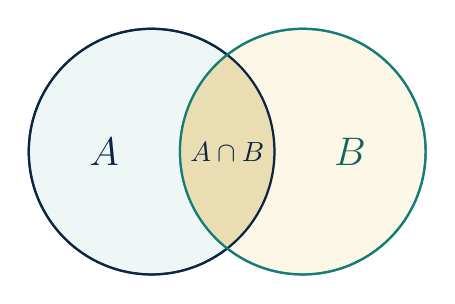
\begin{tikzpicture}[scale=1.2]
    \draw[thick, draw=navy!80, fill=lightteal, fill opacity=0.7] (-0.8, 0) circle (1.3);
    \draw[thick, draw=teal!80, fill=lightgold, fill opacity=0.7] (0.8, 0) circle (1.3);
    \begin{scope}
      \clip (-0.8, 0) circle (1.3);
      \fill[gold!40, fill opacity=0.85] (0.8, 0) circle (1.3);
    \end{scope}
    \draw[thick, draw=navy] (-0.8, 0) circle (1.3);
    \draw[thick, draw=teal] (0.8, 0) circle (1.3);
    \node[navy, font=\bfseries\Large] at (-1.3, 0) {$A$};
    \node[teal!80!black, font=\bfseries\Large] at (1.3, 0) {$B$};
    \node[navy, font=\bfseries] at (0, 0) {$A \cap B$};
  \end{tikzpicture}
  \end{center}
  
  \vspace{1.6cm}
  
  % Metadata card
  \begin{tcolorbox}[
    enhanced,
    colback=white,
    colframe=navy!30,
    boxrule=0.8pt,
    arc=4pt,
    left=16pt, right=16pt, top=14pt, bottom=14pt,
    shadow={2pt}{-2pt}{0pt}{black!10}
  ]
    \renewcommand{\arraystretch}{1.3}
    \begin{tabularx}{\linewidth}{@{}l X@{}}
      \textbf{\color{navy}\small COMPILED BY:} & {\large\bfseries\color{navy} Suleman Ahmed Shuvo} \\
      \textbf{\color{navy}\small ACADEMIC ID:} & {\small\color{darkslate} Roll: 43 \ $\bullet$ \ Batch: CSE-19 \ $\bullet$ \ Session: 2025--2026} \\
      \textbf{\color{navy}\small COURSE:} & {\small\color{teal}\bfseries CSE 1143: Discrete Mathematics (3.00 Credits)} \\
      \textbf{\color{navy}\small DEPARTMENT:} & {\small Dept. of Computer Science \& Engineering} \\
      \textbf{\color{navy}\small INSTITUTION:} & {\small\bfseries Sylhet Engineering College (SEC)} \\
      & {\footnotesize Affiliated with Shahjalal University of Science \& Technology (SUST)} \\
    \end{tabularx}
  \end{tcolorbox}
\end{minipage}
\end{flushleft}
\end{titlepage}
\newpage
\begin{tcolorbox}[
    enhanced,
    colback=lightteal,
    colframe=teal,
    boxrule=0.8pt,
    arc=3pt,
    left=10pt, right=10pt, top=7pt, bottom=7pt
]
\textbf{\color{navy}\large $\bigstar$ SEC TT-01 Tutorial Test Syllabus Guide}\\[2pt]
{\small\textbf{\color{teal}Tutorial Test Date: 7 September, 2026} $\bullet$ \textbf{Dept. of Computer Science \& Engineering}}\\[2pt]
{\small Topics marked with a star (\textbf{\color{gold!90!black}$\bigstar$}) are explicitly included in your upcoming TT-01 syllabus: \textit{Empty / Null Set, Equal Set, Cardinality, Power Set, Set Operations, Venn Diagrams, Domain \& Range, and Reflexive Relations}.}
\end{tcolorbox}
\vspace{10pt}

\begin{center}
{\color{navy}\bfseries\Large\MakeUppercase{Table of Contents}}\\[-3pt]
{\color{gold}\rule{\linewidth}{1.2pt}}
\end{center}
\vspace{4pt}

\begingroup
\hypersetup{linkcolor=navy}
\setcounter{tocdepth}{2}
\makeatletter
\@starttoc{toc}
\makeatother
\endgroup

\newpage


% ==============================================================================
% TITLE HEADER BLOCK
% ==============================================================================


% ==============================================================================
% MODULE 1: THE INTUITIVE FOUNDATIONS OF SETS
% ==============================================================================
\section{The Intuitive Foundation of Sets}

\subsection{Everyday Mental Model: The Shopping Basket}
Imagine walking through a supermarket with a shopping basket. 
\begin{itemize}
    \item You put in an apple, a mango, and a banana. The order in which you tossed them into the basket does not change what you bought.
    \item If you accidentally scan the exact same bottle of milk twice on a checklist, you still only own distinct items of that kind in your mathematical universe.
    \item Everything in your basket is strictly defined: either an item is in the basket, or it is not.
\end{itemize}

\begin{defbox}[Formal Definition: Set]
A \textbf{set} is a well-defined collection of distinct objects. The objects belonging to a set are called its \textbf{elements} or \textbf{members}.
\begin{itemize}
    \item If $x$ is an element of set $A$, we write: \ $\mathbf{x \in A}$ \quad (read: ``$x$ belongs to $A$'').
    \item If $x$ is not an element of set $A$, we write: \ $\mathbf{x \notin A}$ \quad (read: ``$x$ does not belong to $A$'').
\end{itemize}
\end{defbox}

\begin{notebox}[The Two Fundamental Axioms of Elementary Sets]
\begin{enumerate}
    \item \textbf{Order Invariance:} $\{1, 2, 3\} = \{3, 1, 2\} = \{2, 1, 3\}$. Sets do not have a first, second, or last element.
    \item \textbf{Duplication Invariance:} Repeated elements are redundant: $\{1, 1, 2, 3, 3, 3\} = \{1, 2, 3\}$.
\end{enumerate}
\end{notebox}

\subsection{Set Representations}
In computer science and mathematics, we specify sets in two primary ways:

\subsubsection{1. Roster / Listing Form}
All elements are explicitly written out inside curly braces separated by commas:
\[
A = \{2, 4, 6, 8, 10\} \qquad \text{or} \qquad V = \{a, e, i, o, u\}
\]
For infinite or large patterns, an ellipsis ($\dots$) indicates continuation: $E = \{2, 4, 6, 8, \dots\}$.

\subsubsection{2. Set-Builder / Predicate Notation}
Instead of listing elements, we state the exact mathematical rule (predicate $P(x)$) that any candidate element $x$ must satisfy to qualify:
\[
A = \{ x \in U \mid P(x) \} \qquad \text{or} \qquad A = \{ x : P(x) \}
\]
\textit{Read as:} ``The set of all $x$ such that property $P(x)$ is true.''
\begin{itemize}
    \item Example 1: $B = \{x \in \mathbb{Z}^+ \mid x \text{ is odd and } x < 10\} \implies B = \{1, 3, 5, 7, 9\}$.
    \item Example 2: $S = \{x \in \mathbb{R} \mid x^2 - 4 = 0\} \implies S = \{-2, 2\}$.
\end{itemize}

\subsection{Standard Universal Number Systems}
Throughout discrete mathematics and competitive programming, the following blackboard bold symbols are standardized:
\begin{center}
\renewcommand{\arraystretch}{1.2}
\begin{tabularx}{\textwidth}{c l X}
\toprule
\rowcolor{navy!10} \textbf{Symbol} & \textbf{Set Name} & \textbf{Standard Definition / Elements} \\
\midrule
$\mathbb{N}$ & Natural Numbers & $\{0, 1, 2, 3, \dots\}$ \ \textit{(Note: In CS/Rosen, $0 \in \mathbb{N}$)} \\
$\mathbb{Z}$ & Integers & $\{\dots, -3, -2, -1, 0, 1, 2, 3, \dots\}$ \\
$\mathbb{Z}^+$ & Positive Integers & $\{1, 2, 3, 4, \dots\}$ \\
$\mathbb{Q}$ & Rational Numbers & $\{p/q \mid p, q \in \mathbb{Z} \text{ and } q \neq 0\}$ \\
$\mathbb{R}$ & Real Numbers & All rational and irrational numbers (the continuous real line) \\
$\mathbb{C}$ & Complex Numbers & $\{a + bi \mid a, b \in \mathbb{R} \text{ and } i = \sqrt{-1}\}$ \\
\bottomrule
\end{tabularx}
\end{center}

\begin{exambox}{[SEC Final Examination 2022, CSE 103] \ Set Equality, Element Listing \& Finiteness}
\Qlabel
\textbf{1.} Which of these sets are equal: \ $S_1 = \{x, y, z\}$, $S_2 = \{z, y, z, x\}$, $S_3 = \{y, x, y, z\}$, $S_4 = \{y, z, x, y\}$? \hfill\textit{[2]}

\textbf{2.} List the elements of each set where $\mathbb{N} = \{1,2,3,\dots\}$: \ (i) $A = \{x \in \mathbb{N} \mid 3 < x < 9\}$ \ (ii) $B = \{x \in \mathbb{N} \mid x \text{ is even}, x < 11\}$ \ (iii) $C = \{x \in \mathbb{N} \mid 4 + x = 3\}$. \hfill\textit{[1$\times$3]}

\textbf{3.} Determine which of the following sets are finite: (i) Lines parallel to the $x$-axis \ (ii) Letters in the English alphabet \ (iii) Integers which are multiples of 5 \ (iv) Animals living on the earth. \hfill\textit{[2]}
\tcblower
\Alabel
\textbf{1.} By Order/Duplication Invariance, all repeat and reorder to $\{x,y,z\}$ $\implies \mathbf{S_1=S_2=S_3=S_4}$.

\textbf{2.} $\mathbf{A = \{4,5,6,7,8\}}$; \quad $\mathbf{B = \{2,4,6,8,10\}}$; \quad $C: x=-1\notin\mathbb{N} \implies \mathbf{C=\emptyset}$.

\textbf{3.} (i) \textbf{Infinite} \quad (ii) \textbf{Finite} ($|S|=26$) \quad (iii) \textbf{Infinite} \quad (iv) \textbf{Finite} (population is bounded at any instant).
\end{exambox}

% ==============================================================================
% MODULE 2: SPECIAL SETS, SUBSETS & THE GREAT TRAP
% ==============================================================================
\section{Special Sets, Subsets \& The Great Trap: \texorpdfstring{$\in$}{in} vs. \texorpdfstring{$\subseteq$}{subset}}

\subsection{\texorpdfstring{$\bigstar$ }{*}Special Types of Sets: Empty / Null Set \& Universal Set}
\noindent{\footnotesize\color{teal}\textbf{$\bigstar$ TT-01 Syllabus Topic (7 Sept 2026):} \textit{Empty Set or Null Set ($\emptyset$)}}\\[3pt]
\begin{enumerate}
    \item \textbf{Universal Set ($\mathcal{U}$ or $U$):} The overarching domain containing all possible objects under current discussion.
    \item \textbf{Empty Set / Null Set ($\emptyset$ or $\{\}$):} A set containing zero elements ($|\emptyset| = 0$).
    \item \textbf{Singleton Set:} Any set containing exactly one single element, e.g., $\{42\}$ or $\{\emptyset\}$.
\end{enumerate}

\begin{exambox}{[SEC TT-01 / Final Examination 2024, CSE 0541 1143] \ Set Definition \& Classification of Sets}
\Qlabel
Define a set and list the different types of sets. Give an example for each type. \hfill\textit{[2+4]}
\tcblower
\Alabel
A set is a well-defined collection of distinct objects (elements).
\begin{itemize}
    \item \textbf{Finite Set:} Contains a countable number of elements. Example: $A = \{2, 4, 6\}$, $|A| = 3$.
    \item \textbf{Infinite Set:} Elements cannot be exhausted. Example: $\mathbb{N} = \{1, 2, 3, \dots\}$.
    \item \textbf{Empty / Null Set ($\emptyset$):} Contains zero elements ($|\emptyset| = 0$). Example: $\{x \in \mathbb{R} \mid x^2 + 1 = 0\} = \emptyset$.
    \item \textbf{Singleton Set:} Contains exactly one element. Example: $\{0\}$ or $\{\emptyset\}$.
    \item \textbf{Universal Set ($U$):} Contains all objects under discussion. Example: $U = \mathbb{R}$.
    \item \textbf{Equal Sets ($A = B$):} Contain identical members. Example: $\{1, 2\} = \{2, 1, 1\}$.
    \item \textbf{Subset ($A \subseteq B$):} $\forall x (x \in A \implies x \in B)$. Example: $\{1, 2\} \subseteq \{1, 2, 3\}$.
    \item \textbf{Power Set ($\mathcal{P}(S)$):} Set of all subsets. Example: $\mathcal{P}(\{1\}) = \{\emptyset, \{1\}\}$.
\end{itemize}
\end{exambox}

\begin{warningbox}[The Classic Empty Set Trap: $\emptyset$ vs. $\{\emptyset\}$]
A common beginner mistake is confusing the empty set $\emptyset$ with the singleton set $\{\emptyset\}$.
\begin{itemize}
    \item $\mathbf{\emptyset}$: An empty plastic box. It contains zero items inside. Cardinality $|\emptyset| = 0$.
    \item $\mathbf{\{\emptyset\}}$: A plastic box that has an empty plastic box placed inside it. It contains \textbf{one object} (which happens to be an empty box!). Cardinality $|\{\emptyset\}| = 1$.
    \item Therefore: $\mathbf{\emptyset \neq \{\emptyset\}}$ and $|\emptyset| \neq |\{\emptyset\}|$.
\end{itemize}
\end{warningbox}

\subsection{\texorpdfstring{$\bigstar$ }{*}Subsets, Strict Subsets and Equal Sets}
\noindent{\footnotesize\color{teal}\textbf{$\bigstar$ TT-01 Syllabus Topic (7 Sept 2026):} \textit{Equal Sets ($A = B \iff A \subseteq B \land B \subseteq A$)}}\\[3pt]
\begin{defbox}[Subset ($\subseteq$) and Proper Subset ($\subset$)]
Let $A$ and $B$ be two arbitrary sets:
\begin{itemize}
    \item $\mathbf{A \subseteq B}$ ($A$ is a subset of $B$) if and only if every element of $A$ is also an element of $B$:
    \[
    \mathbf{A \subseteq B \iff \forall x (x \in A \implies x \in B)}
    \]
    \item $\mathbf{A \subset B}$ or $\mathbf{A \subsetneq B}$ ($A$ is a \textbf{proper} or \textbf{strict} subset of $B$) if $A \subseteq B$ and $A \neq B$ (i.e., $B$ contains at least one element not present in $A$).
    \item \textbf{Set Equality ($A = B$):} Two sets are equal if and only if they contain the exact same elements:
    \[
    \mathbf{A = B \iff (A \subseteq B \land B \subseteq A)}
    \]
\end{itemize}
\end{defbox}

\begin{theorembox}[Theorem: The Empty Set is a Subset of Every Set]
\textbf{Proposition:} For any arbitrary set $S$, $\mathbf{\emptyset \subseteq S}$.\\
\textbf{Proof (Vacuous Truth):}
By definition of subset, $\emptyset \subseteq S$ means:
\[
\forall x (x \in \emptyset \implies x \in S)
\]
Because the empty set $\emptyset$ has no elements, the premise $x \in \emptyset$ is \textbf{always False} for every possible $x$. In classical logic, any conditional statement with a False antecedent ($F \implies P$) is \textbf{vacuously True}. Thus, $\emptyset \subseteq S$ holds universally for every set $S$. $\blacksquare$
\end{theorembox}

\subsection{The Membership (\texorpdfstring{$\in$}{in}) vs. Inclusion (\texorpdfstring{$\subseteq$}{subset}) Dissection}
The distinction between element membership and subset inclusion represents one of the most common conceptual pitfalls where students make errors.

\begin{defbox}[The Gold Rule of \texorpdfstring{$\in$}{in} vs. \texorpdfstring{$\subseteq$}{subset}]
\begin{itemize}
    \item $\mathbf{x \in A}$ is a relationship between an \textbf{individual element} and a set. $x$ must literally appear as an item inside $A$'s braces.
    \item $\mathbf{S \subseteq A}$ is a relationship between \textbf{two sets}. Every element inside $S$ must belong to $A$.
    \item \textbf{The Braces Conversion Rule:} If $x \in A$, then wrapping $x$ in a set gives $\{x\} \subseteq A$.
\end{itemize}
\end{defbox}

\begin{examplebox}[Master Example: Analyzing $A = \{1, 2, \{3\}, \{4, 5\}, \emptyset\}$]
Consider the set: $A = \{1, \, 2, \, \{3\}, \, \{4, 5\}, \, \emptyset\}$.
\begin{center}
\renewcommand{\arraystretch}{1.3}
\begin{tabularx}{\textwidth}{l c X}
\toprule
\rowcolor{navy!10} \textbf{Statement} & \textbf{Truth Value} & \textbf{Rigorous Mathematical Explanation} \\
\midrule
$1 \in A$ & \textbf{True} & $1$ is an explicitly listed member of $A$. \\
$\{1\} \in A$ & \textbf{False} & $\{1\}$ is not in the set; only the naked integer $1$ is present. \\
$\{1\} \subseteq A$ & \textbf{True} & The single element inside $\{1\}$, namely $1$, belongs to $A$. \\
$3 \in A$ & \textbf{False} & $3$ is locked inside a nested subset; it is not a direct member. \\
$\{3\} \in A$ & \textbf{True} & The set $\{3\}$ is itself a direct element inside $A$. \\
$\{3\} \subseteq A$ & \textbf{False} & The element inside $\{3\}$ is $3$, but $3 \notin A$. \\
$\{\{3\}\} \subseteq A$ & \textbf{True} & The element inside $\{\{3\}\}$ is $\{3\}$, and $\{3\} \in A$. \\
$\emptyset \in A$ & \textbf{True} & $\emptyset$ is explicitly written inside $A$ as an element. \\
$\emptyset \subseteq A$ & \textbf{True} & The empty set is vacuously a subset of every set. \\
$\{\emptyset\} \subseteq A$ & \textbf{True} & The element inside $\{\emptyset\}$ is $\emptyset$, and $\emptyset \in A$. \\
\bottomrule
\end{tabularx}
\end{center}
\end{examplebox}

% ==============================================================================
% MODULE 3: CARDINALITY & POWER SETS
% ==============================================================================
\section{Cardinality \& The Power Set Explosion}

\subsection{\texorpdfstring{$\bigstar$ }{*}Cardinality of a Set}
\noindent{\footnotesize\color{teal}\textbf{$\bigstar$ TT-01 Syllabus Topic (7 Sept 2026):} \textit{Cardinality of a Set ($|S| = n$)}}\\[3pt]
\begin{defbox}[Cardinality]
If $S$ is a finite set containing $n$ distinct elements (where $n \in \mathbb{N}$), we say $S$ is a finite set with \textbf{cardinality} $n$, denoted by $\mathbf{|S| = n}$.
\begin{itemize}
    \item $|\emptyset| = 0$
    \item $|\{a, b, c\}| = 3$
    \item $|\{1, \{2, 3\}, 4\}| = 3$ \ \textit{(the pair $\{2, 3\}$ counts as 1 single composite element)}.
\end{itemize}
\end{defbox}

\begin{exambox}{[SEC Final Examination 2022, CSE 103] \ Cardinal Number of Sets}
\Qlabel
Find the cardinal number of each of the following sets: \ (i) $A = \{a, b, c, \dots, y, z\}$ \quad (ii) $B = \{x \mid x \in \mathbb{N}, \, x^2 = 5\}$ \quad (iii) $C = \{10, 20, 30, 40, \dots\}$ \quad (iv) $D = \{6, 7, 8, 9, \dots\}$. \hfill\textit{[2]}
\tcblower
\Alabel
\begin{itemize}
    \item $A$ = 26 lower-case letters $\implies \mathbf{|A| = 26}$.
    \item $x^2=5 \implies x=\pm\sqrt5 \notin \mathbb{N} \implies B=\emptyset \implies \mathbf{|B|=0}$.
    \item $C=\{10k \mid k\in\mathbb{Z}^+\} \implies \mathbf{|C| = \aleph_0}$ (Countably Infinite).
    \item $D=\{n\in\mathbb{N}\mid n\ge6\} \implies \mathbf{|D| = \aleph_0}$ (Countably Infinite).
\end{itemize}
\end{exambox}

\subsection{\texorpdfstring{$\bigstar$ }{*}The Power Set (\texorpdfstring{$\mathcal{P}(S)$}{P(S)}) \& Cardinality \texorpdfstring{$2^n$}{2\textasciicircum n}}
\noindent{\footnotesize\color{teal}\textbf{$\bigstar$ TT-01 Syllabus Topic (7 Sept 2026):} \textit{Power Set and Cardinality Theorem $|\mathcal{P}(S)| = 2^n$}}\\[3pt]
\begin{defbox}[Power Set]
Given a set $S$, the \textbf{power set} of $S$, denoted by $\mathbf{\mathcal{P}(S)}$ or $\mathbf{2^S}$, is the set of \textbf{all possible subsets} of $S$:
\[
\mathbf{\mathcal{P}(S) = \{ X \mid X \subseteq S \}}
\]
\end{defbox}

\begin{theorembox}[Theorem: Cardinality of the Power Set]
\textbf{Proposition:} If $|S| = n$, then $|\mathcal{P}(S)| = 2^n$.\\
\textbf{Intuitive Proof (The Binary Decision Tree):}\\
To construct any arbitrary subset $X \subseteq S$, we inspect each of the $n$ elements in $S$ one by one. For each element $x_i$, we have exactly \textbf{2 choices}:
\[
\text{Choice: } \begin{cases} \text{Include } x_i \text{ in } X & (\text{Bit } 1) \\ \text{Exclude } x_i \text{ from } X & (\text{Bit } 0) \end{cases}
\]
By the Fundamental Counting Rule of Combinatorics:
\[
\underbrace{2 \times 2 \times 2 \times \dots \times 2}_{n \text{ decisions}} = 2^n \text{ unique subsets}. \quad \blacksquare
\]
\end{theorembox}

\begin{examplebox}[Tracing All Subsets of $S = \{a, b, c\}$]
Let $S = \{a, b, c\}$. Since $|S| = 3$, $|\mathcal{P}(S)| = 2^3 = 8$ subsets:
\[
\mathcal{P}(S) = \big\{ \emptyset, \ \{a\}, \ \{b\}, \ \{c\}, \ \{a, b\}, \ \{a, c\}, \ \{b, c\}, \ \{a, b, c\} \big\}
\]
\end{examplebox}

\begin{center}
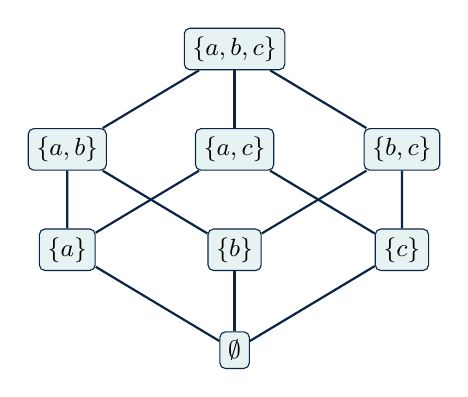
\begin{tikzpicture}[scale=0.85, every node/.style={draw=navy, fill=lightteal, rounded corners=2pt, font=\bfseries\small, inner sep=3pt}]
  % Hasse Diagram for Power Set of 3 elements
  \node (top) at (0, 3) {$\{a, b, c\}$};
  
  \node (ab) at (-2.5, 1.5) {$\{a, b\}$};
  \node (ac) at (0, 1.5) {$\{a, c\}$};
  \node (bc) at (2.5, 1.5) {$\{b, c\}$};
  
  \node (a) at (-2.5, 0) {$\{a\}$};
  \node (b) at (0, 0) {$\{b\}$};
  \node (c) at (2.5, 0) {$\{c\}$};
  
  \node (bot) at (0, -1.5) {$\emptyset$};
  
  \draw[navy, thick] (bot) -- (a);
  \draw[navy, thick] (bot) -- (b);
  \draw[navy, thick] (bot) -- (c);
  
  \draw[navy, thick] (a) -- (ab);
  \draw[navy, thick] (a) -- (ac);
  \draw[navy, thick] (b) -- (ab);
  \draw[navy, thick] (b) -- (bc);
  \draw[navy, thick] (c) -- (ac);
  \draw[navy, thick] (c) -- (bc);
  
  \draw[navy, thick] (ab) -- (top);
  \draw[navy, thick] (ac) -- (top);
  \draw[navy, thick] (bc) -- (top);
\end{tikzpicture}\\[3pt]
{\small\textit{\color{navy}\textbf{Figure 1:} Hasse subset-inclusion lattice for the Boolean algebra $\mathcal{P}(\{a, b, c\})$.}}
\end{center}

\subsection{Recursive Power Sets of the Null Set}
What happens when we repeatedly apply the power set operator to the empty set?
\begin{enumerate}
    \item Start with $\emptyset$: $|\emptyset| = 0$.
    \item $\mathcal{P}(\emptyset) = \{\emptyset\}$. Cardinality $= 2^0 = \mathbf{1}$.
    \item $\mathcal{P}(\mathcal{P}(\emptyset)) = \mathcal{P}(\{\emptyset\}) = \{\emptyset, \{\emptyset\}\}$. Cardinality $= 2^1 = \mathbf{2}$.
    \item $\mathcal{P}(\mathcal{P}(\mathcal{P}(\emptyset))) = \big\{ \emptyset, \, \{\emptyset\}, \, \{\{\emptyset\}\}, \, \{\emptyset, \{\emptyset\}\} \big\}$. Cardinality $= 2^2 = \mathbf{4}$.
    \item $\big|\mathcal{P}\big(\mathcal{P}\big(\mathcal{P}\big(\mathcal{P}(\emptyset)\big)\big)\big)\big| = 2^4 = \mathbf{16}$.
\end{enumerate}

% ==============================================================================
% MODULE 4: CARTESIAN PRODUCT
% ==============================================================================
\section{Cartesian Product \& Ordered \texorpdfstring{$n$-Tuples}{n-Tuples}}

\subsection{Ordered Pairs vs. Unordered Sets}
In a set, order is ignored: $\{1, 2\} = \{2, 1\}$. But in computer programming (such as coordinates, database tables, or key-value tuples), position matters! 
An \textbf{ordered pair} $(a, b)$ has a designated first element $a$ and second element $b$:
\[
(a, b) = (c, d) \iff (a = c \ \land \ b = d)
\]

\begin{defbox}[Cartesian Product (\texorpdfstring{$A \times B$}{A x B})]
The \textbf{Cartesian product} of two sets $A$ and $B$, denoted by $\mathbf{A \times B}$, is the set of all ordered pairs $(a, b)$ where $a \in A$ and $b \in B$:
\[
\mathbf{A \times B = \{ (a, b) \mid a \in A \land b \in B \}}
\]
\end{defbox}

\begin{notebox}[Properties of the Cartesian Product]
\begin{itemize}
    \item \textbf{Cardinality Rule:} If $|A| = m$ and $|B| = n$, then: $\mathbf{|A \times B| = m \cdot n}$.
    \item \textbf{Non-Commutative:} In general, $\mathbf{A \times B \neq B \times A}$ (unless $A = B$ or one of them is $\emptyset$).
    \item \textbf{Null Absorption:} $\mathbf{A \times \emptyset = \emptyset \times A = \emptyset}$ (since no ordered pair can be formed with an element from $\emptyset$).
\end{itemize}
\end{notebox}

\begin{examplebox}[Cartesian Product Calculation]
Let $A = \{1, 2\}$ and $B = \{x, y, z\}$.
\begin{itemize}
    \item $A \times B = \big\{ (1, x), (1, y), (1, z), (2, x), (2, y), (2, z) \big\}$. Cardinality: $2 \times 3 = 6$.
    \item $B \times A = \big\{ (x, 1), (x, 2), (y, 1), (y, 2), (z, 1), (z, 2) \big\}$.
    \item Observe that $(1, x) \neq (x, 1)$, confirming $A \times B \neq B \times A$.
\end{itemize}
\end{examplebox}

\begin{exambox}{[SEC TT-01, CSE 103, 2022] \ Cartesian Product, Set Intersection \& Floor/Ceiling}
\Qlabel
(a) Let $A = \{1, 2, 3\}$, $B = \{a, b, c, d\}$ and $C = \{c, d\}$. Find: $(A \times B) \cap (A \times C)$ and $(B \cap C)$. \hfill\textit{[5]}\\
(b) Find: (i) $\lfloor 7.5 \rfloor$, $\lfloor -7.5 \rfloor$, $\lfloor -18 \rfloor$; \ (ii) $\lceil 7.5 \rceil$, $\lceil -7.5 \rceil$, $\lceil -18 \rceil$. \hfill\textit{[5]}
\tcblower
\Alabel
(a) $B \cap C = \mathbf{\{c, d\}}$. By distributivity, $(A \times B) \cap (A \times C) = A \times (B \cap C)$
\[
\mathbf{= \{(1, c), (1, d), (2, c), (2, d), (3, c), (3, d)\}}
\]
(b) $\lfloor 7.5 \rfloor = \mathbf{7}$, $\lfloor -7.5 \rfloor = \mathbf{-8}$, $\lfloor -18 \rfloor = \mathbf{-18}$; \quad $\lceil 7.5 \rceil = \mathbf{8}$, $\lceil -7.5 \rceil = \mathbf{-7}$, $\lceil -18 \rceil = \mathbf{-18}$.
\end{exambox}

\newpage
\subsection{\texorpdfstring{$\bigstar$ }{*}Relations Introduction: Domain, Range \& Reflexive Relations}
\noindent{\footnotesize\color{teal}\textbf{$\bigstar$ TT-01 Syllabus Topic (7 Sept 2026):} \textit{Binary Relations, Domain, Range, and Reflexivity}}\\[4pt]

\begin{defbox}[Binary Relation, Domain \& Range]
Let $A$ and $B$ be sets. A \textbf{binary relation} $R$ from $A$ to $B$ is any subset of the Cartesian product $A \times B$:
\[
R \subseteq A \times B
\]
If $(a, b) \in R$, we write $a \, R \, b$ (read: ``$a$ is related to $b$''). If $A = B$, $R$ is called a relation on $A$.
\begin{itemize}
    \item \textbf{Domain of $R$ ($\operatorname{Dom}(R)$):} The set of all first coordinates from the ordered pairs in $R$:
    \[
    \operatorname{Dom}(R) = \{ a \in A \mid \exists b \in B, \, (a, b) \in R \} \subseteq A
    \]
    \item \textbf{Range of $R$ ($\operatorname{Range}(R)$):} The set of all second coordinates from the ordered pairs in $R$:
    \[
    \operatorname{Range}(R) = \{ b \in B \mid \exists a \in A, \, (a, b) \in R \} \subseteq B
    \]
\end{itemize}
\end{defbox}

\begin{defbox}[Core Relation Properties: Reflexive, Symmetric, Transitive \& Equivalence]
Let $R$ be a binary relation on a set $A$:
\begin{itemize}
    \item \textbf{Reflexive:} $\forall a \in A, \ (a, a) \in R$. \quad (Matrix diagonal $m_{ii} = 1$; Digraph has self-loops on all vertices).
    \item \textbf{Symmetric:} $\forall x, y \in A, \ (x, y) \in R \implies (y, x) \in R$. \quad (Matrix satisfies $M = M^T$).
    \item \textbf{Antisymmetric:} $\forall x, y \in A, \ ((x, y) \in R \land (y, x) \in R) \implies x = y$.
    \item \textbf{Transitive:} $\forall x, y, z \in A, \ ((x, y) \in R \land (y, z) \in R) \implies (x, z) \in R$.
    \item \textbf{Equivalence Relation:} A relation $R$ that is simultaneously \textbf{reflexive}, \textbf{symmetric}, and \textbf{transitive}.
\end{itemize}
\end{defbox}

\begin{exambox}{[SEC Final Examination 2023, CSE 143] \ Relation Matrix, Arrow Diagram, Inverse, Domain \& Range}
\Qlabel
Given $A = \{1, 2, 3, 4\}$ and $B = \{x, y, z\}$. Let $R = \{(1, y), (1, z), (3, y), (4, x), (4, z)\}$ be a relation from $A$ to $B$. (i) Determine the matrix of the relation. (ii) Draw the arrow diagram of $R$. (iii) Find the inverse relation $R^{-1}$. (iv) Determine the domain and range of $R$. \hfill\textit{[4]}
\tcblower
\Alabel
\textbf{(i) Matrix} (rows $A=(1,2,3,4)$, columns $B=(x,y,z)$):
\[
M_R = \begin{pmatrix}
0 & 1 & 1 \\
0 & 0 & 0 \\
0 & 1 & 0 \\
1 & 0 & 1
\end{pmatrix}
\]
\textbf{(ii) Arrow Diagram:}
\begin{center}
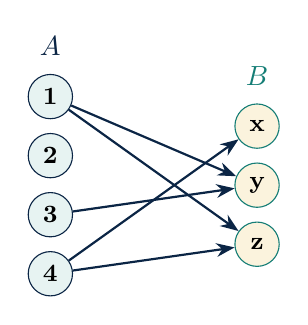
\begin{tikzpicture}[scale=0.75, >=Stealth]
  \foreach \y/\lab in {3/1, 2/2, 1/3, 0/4} {
    \node[circle, draw=navy, fill=lightteal, font=\bfseries\small, inner sep=2pt, minimum size=16pt] (a\lab) at (0, \y) {\lab};
  }
  \node[above=3pt of a1, font=\bfseries\color{navy}] {$A$};
  \foreach \y/\lab in {2.5/x, 1.5/y, 0.5/z} {
    \node[circle, draw=teal, fill=lightgold, font=\bfseries\small, inner sep=2pt, minimum size=16pt] (b\lab) at (3.5, \y) {\lab};
  }
  \node[above=3pt of bx, font=\bfseries\color{teal}] {$B$};
  \draw[->, thick, navy] (a1) -- (by);
  \draw[->, thick, navy] (a1) -- (bz);
  \draw[->, thick, navy] (a3) -- (by);
  \draw[->, thick, navy] (a4) -- (bx);
  \draw[->, thick, navy] (a4) -- (bz);
\end{tikzpicture}
\end{center}
\textbf{(iii)} $R^{-1} = \mathbf{\{(y,1),(z,1),(y,3),(x,4),(z,4)\}}$. \quad
\textbf{(iv)} $\operatorname{Dom}(R) = \mathbf{\{1,3,4\}}$, \ $\operatorname{Range}(R) = \mathbf{\{x,y,z\}}$.
\end{exambox}

\begin{exambox}{[SEC Final Examination 2023, CSE 143] \ Digraph Model of a Binary Relation}
\Qlabel
Define Relation. Find the relation $R$ determined by the directed graph below: \hfill\textit{[1+2]}
\begin{center}
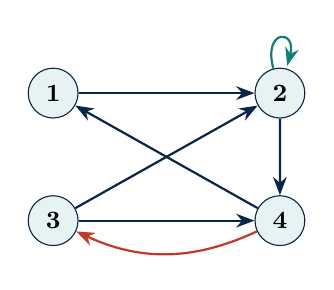
\begin{tikzpicture}[scale=0.9, >=Stealth, every node/.style={circle, draw=navy, fill=lightteal, font=\bfseries\small, inner sep=2pt, minimum size=18pt}]
  \node (n1) at (0, 1.8) {1};
  \node (n2) at (3.2, 1.8) {2};
  \node (n3) at (0, 0) {3};
  \node (n4) at (3.2, 0) {4};
  \draw[->, thick, navy] (n1) -- (n2);
  \path[->, thick, teal] (n2) edge [loop above] (n2);
  \draw[->, thick, navy] (n2) -- (n4);
  \draw[->, thick, navy] (n3) -- (n2);
  \draw[->, thick, navy] (n3) -- (n4);
  \draw[->, thick, navy] (n4) -- (n1);
  \draw[->, thick, coral] (n4) to[bend left=25] (n3);
\end{tikzpicture}
\end{center}
\tcblower
\Alabel
\textbf{Definition of Relation:} A binary relation $R$ from set $A$ to set $B$ is any mathematical subset of the Cartesian product $A \times B$ ($R \subseteq A \times B$). When $A = B$, $R$ is a relation on $A$.\\[4pt]
\textbf{Extracting Directed Edges into Ordered Pairs:}
We inspect the directed arrows emanating from each vertex in vertex set $V = \{1, 2, 3, 4\}$:
\begin{itemize}
    \item From vertex $1$: edge to $2 \implies (1, 2)$.
    \item From vertex $2$: self-loop at $2$ and edge to $4 \implies (2, 2), (2, 4)$.
    \item From vertex $3$: edges to $2$ and $4 \implies (3, 2), (3, 4)$.
    \item From vertex $4$: edges to $1$ and $3$ (curved) $\implies (4, 1), (4, 3)$.
\end{itemize}
Thus, the binary relation represented by the directed graph is:
\[
\mathbf{R = \big\{ (1, 2), \, (2, 2), \, (2, 4), \, (3, 2), \, (3, 4), \, (4, 1), \, (4, 3) \big\}} \qquad (|R| = 7 \text{ pairs}).
\]
\end{exambox}

\begin{exambox}{[SEC Final Examination 2023, CSE 143] \ Reflexive, Symmetric \& Transitive Closures}
\Qlabel
Consider the relation $R = \{(a,a), (a,b), (b,c), (c,c)\}$ on the set $A = \{a,b,c\}$. Find: (i) $\operatorname{reflexive}(R)$; (ii) $\operatorname{symmetric}(R)$; (iii) $\operatorname{transitive}(R)$. \hfill\textit{[3]}
\tcblower
\Alabel
The \textbf{closure} of a relation $R$ with respect to property $P$ is the smallest relation $R' \supseteq R$ that satisfies property $P$:
\begin{enumerate}
    \item \textbf{(i) Reflexive Closure ($\operatorname{reflexive}(R) = R \cup \Delta_A$):}
    A relation on $A=\{a,b,c\}$ is reflexive iff it contains the full diagonal $\Delta_A = \{(a,a), (b,b), (c,c)\}$. In $R$, the self-loop $(b,b)$ is missing. Adding it yields:
    \[
    \mathbf{\operatorname{reflexive}(R) = \{(a,a), (a,b), (b,b), (b,c), (c,c)\}}
    \]
    \item \textbf{(ii) Symmetric Closure ($\operatorname{symmetric}(R) = R \cup R^{-1}$):}
    We must add $(y,x)$ for every $(x,y) \in R$. The pairs $(a,b)$ and $(b,c)$ lack reverse pairs $(b,a)$ and $(c,b)$:
    \[
    \mathbf{\operatorname{symmetric}(R) = \{(a,a), (a,b), (b,a), (b,c), (c,b), (c,c)\}}
    \]
    \item \textbf{(iii) Transitive Closure ($\operatorname{transitive}(R) = R^+$):}
    We identify all path chains $(x,y) \in R \land (y,z) \in R \implies (x,z) \in R$.
    Here, $(a,b) \in R$ and $(b,c) \in R$, which requires the transitive shortcut pair $\mathbf{(a,c)}$. No further composite chains exist:
    \[
    \mathbf{\operatorname{transitive}(R) = \{(a,a), (a,b), (a,c), (b,c), (c,c)\}}
    \]
\end{enumerate}
\end{exambox}

\begin{exambox}{[SEC TT-01 / Final Examination 2024, CSE 0541 1143] \ Tracing Relations on $A = \{1, 2, 3, 4\}$}
\Qlabel
Consider the five relations on $A=\{1,2,3,4\}$: $R=\{(1,1),(1,2),(2,3),(1,3),(4,4)\}$; $S=\{(1,1),(1,2),(2,1),(2,2),(3,3),(4,4)\}$; $T=\{(1,3),(2,1)\}$; $U=A\times A$; $V=\emptyset$. Determine with reason whether each is (i) Reflexive (ii) Symmetric (iii) Transitive. Define Equivalence relation with example. \hfill\textit{[6+2]}
\tcblower
\Alabel
\begin{itemize}
    \item $\mathbf{R}$: Reflexive --- \textbf{No} (missing $(2,2),(3,3)$). Symmetric --- \textbf{No} ($(1,2)\in R$, $(2,1)\notin R$). Transitive --- \textbf{Yes}.
    \item $\mathbf{S}$: Reflexive --- \textbf{Yes}. Symmetric --- \textbf{Yes}. Transitive --- \textbf{Yes} $\implies$ \textbf{Equivalence Relation}.
    \item $\mathbf{T}$: Reflexive --- \textbf{No} (no self-loops). Symmetric --- \textbf{No}. Transitive --- \textbf{Yes} (vacuously; no chaining pairs).
    \item $\mathbf{U=A\times A}$: Reflexive, Symmetric, Transitive --- \textbf{all Yes} (contains every pair).
    \item $\mathbf{V=\emptyset}$: Reflexive --- \textbf{No} (since $A\neq\emptyset$). Symmetric, Transitive --- \textbf{Yes} (vacuously true).
\end{itemize}
\textbf{Equivalence Relation:} $R$ is an equivalence relation iff reflexive, symmetric, \emph{and} transitive --- e.g., congruence mod $m$ on $\mathbb{Z}$, or $S$ above.
\end{exambox}

\newpage
\begin{exambox}{[SEC TT-01 / Final Examination 2024, CSE 0541 1143] \ Divisibility Relation \& Directed Graph}
\Qlabel
Let $A = \{1, 2, 3, 4, 5, 6\}$ and let $R$ be the relation on $A$: $R = \{(x,y) \mid x \text{ divides } y\}$. (i) Write $R$ as a set of ordered pairs. (ii) Draw its directed graph. \hfill\textit{[2+3]}
\tcblower
\Alabel
\begin{align*}
R = \{ &(1, 1), (1, 2), (1, 3), (1, 4), (1, 5), (1, 6), \\
       &(2, 2), (2, 4), (2, 6), \ (3, 3), (3, 6), \ (4, 4), \ (5, 5), \ (6, 6) \} \qquad (|R| = 14)
\end{align*}
\begin{center}
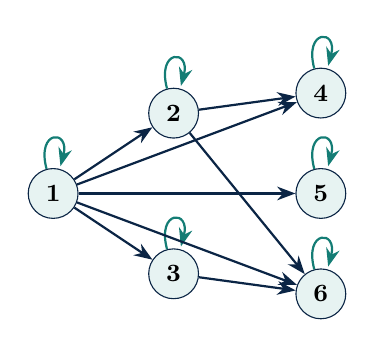
\begin{tikzpicture}[scale=0.85, >=Stealth, every node/.style={circle, draw=navy, fill=lightteal, font=\bfseries\small, inner sep=2pt, minimum size=18pt}]
  \node (n1) at (0, 0) {1};
  \node (n2) at (1.8, 1.2) {2};
  \node (n3) at (1.8, -1.2) {3};
  \node (n4) at (4.0, 1.5) {4};
  \node (n5) at (4.0, 0) {5};
  \node (n6) at (4.0, -1.5) {6};
  \foreach \v in {1, 2, 3, 4, 5, 6} {
    \path[->, thick, teal] (n\v) edge [loop above] (n\v);
  }
  \foreach \v in {2, 3, 4, 5, 6} {
    \path[->, thick, navy] (n1) edge (n\v);
  }
  \path[->, thick, navy] (n2) edge (n4);
  \path[->, thick, navy] (n2) edge (n6);
  \path[->, thick, navy] (n3) edge (n6);
\end{tikzpicture}
\end{center}
\end{exambox}

\begin{exambox}{[SEC TT-02, CSE 103, 2022] \ Matrix Representation: Reflexive, Symmetric \& Antisymmetric}
\Qlabel
Determine whether the relation represented by the matrix below is reflexive, symmetric, or antisymmetric?
\[
M = \begin{pmatrix}
1 & 1 & 1 & 0 \\
0 & 1 & 0 & 0 \\
0 & 0 & 1 & 1 \\
1 & 0 & 0 & 1
\end{pmatrix}
\]
\hfill\textit{[3]}
\tcblower
\Alabel
\textbf{Reflexive:} all diagonal entries $m_{11}=m_{22}=m_{33}=m_{44}=1$ $\implies$ \textbf{Yes}. \quad
\textbf{Symmetric:} $m_{12}=1$ but $m_{21}=0 \implies M \neq M^T \implies$ \textbf{No}. \quad
\textbf{Antisymmetric:} every off-diagonal $1$ ($m_{12},m_{13},m_{34},m_{41}$) has its mirror entry $0$ $\implies$ \textbf{Yes}.
\end{exambox}

\begin{exambox}{[SEC TT-02, CSE 103, 2022] \ Function vs. Relation}
\Qlabel
Is every function a relation and vice versa? \hfill\textit{[3]}
\tcblower
\Alabel
\textbf{Every function is a relation} --- $f:A\to B$ is simply $R\subseteq A\times B$ where each $a\in A$ pairs with exactly \emph{one} $b\in B$. \quad
\textbf{Not every relation is a function} --- a relation may map one $a$ to several $b$'s (e.g., $\{(1,2),(1,3)\}$) or leave some $a$ unassigned.
\end{exambox}

% ==============================================================================
% MODULE 5: SET OPERATIONS & VENN DIAGRAMS
% ==============================================================================
\newpage
\section{\texorpdfstring{$\bigstar$ }{*}Fundamental Set Operations \& Venn Diagrams}
\noindent{\footnotesize\color{teal}\textbf{$\bigstar$ TT-01 Syllabus Topic (7 Sept 2026):} \textit{Set Operations and Venn Diagrams}}\\[4pt]

Venn diagrams provide a visual geometry for Boolean set logic inside a bounding Universal set $\mathcal{U}$.

\begin{center}
\begin{tabular}{ccc}
% 1. Union
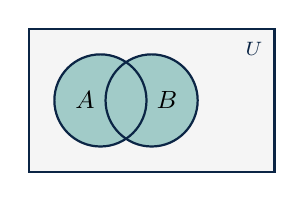
\begin{tikzpicture}[scale=0.65]
  \draw[thick, draw=navy, fill=gray!8] (-1.9,-1.4) rectangle (2.9,1.4);
  \node[navy, font=\bfseries\scriptsize] at (2.5,1.0) {$U$};
  \fill[teal!40] (-0.5,0) circle (0.9);
  \fill[teal!40] (0.5,0) circle (0.9);
  \draw[thick, draw=navy] (-0.5,0) circle (0.9);
  \draw[thick, draw=navy] (0.5,0) circle (0.9);
  \node[font=\bfseries\small] at (-0.8,0) {$A$};
  \node[font=\bfseries\small] at (0.8,0) {$B$};
\end{tikzpicture} &
% 2. Intersection
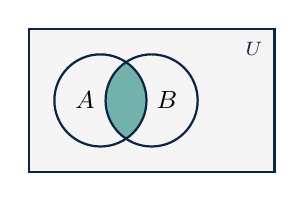
\begin{tikzpicture}[scale=0.65]
  \draw[thick, draw=navy, fill=gray!8] (-1.9,-1.4) rectangle (2.9,1.4);
  \node[navy, font=\bfseries\scriptsize] at (2.5,1.0) {$U$};
  \begin{scope}
    \clip (-0.5,0) circle (0.9);
    \fill[teal!60] (0.5,0) circle (0.9);
  \end{scope}
  \draw[thick, draw=navy] (-0.5,0) circle (0.9);
  \draw[thick, draw=navy] (0.5,0) circle (0.9);
  \node[font=\bfseries\small] at (-0.8,0) {$A$};
  \node[font=\bfseries\small] at (0.8,0) {$B$};
\end{tikzpicture} &
% 3. Difference A - B
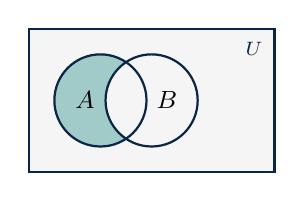
\begin{tikzpicture}[scale=0.65]
  \draw[thick, draw=navy, fill=gray!8] (-1.9,-1.4) rectangle (2.9,1.4);
  \node[navy, font=\bfseries\scriptsize] at (2.5,1.0) {$U$};
  \begin{scope}
    \clip (-0.5,0) circle (0.9);
    \fill[teal!40] (-0.5,0) circle (0.9);
    \fill[gray!8] (0.5,0) circle (0.9);
  \end{scope}
  \draw[thick, draw=navy] (-0.5,0) circle (0.9);
  \draw[thick, draw=navy] (0.5,0) circle (0.9);
  \node[font=\bfseries\small] at (-0.8,0) {$A$};
  \node[font=\bfseries\small] at (0.8,0) {$B$};
\end{tikzpicture} \\
\textbf{(a) Union: } $A \cup B$ & \textbf{(b) Intersection: } $A \cap B$ & \textbf{(c) Difference: } $A \setminus B$ \\[6pt]

% 4. Complement
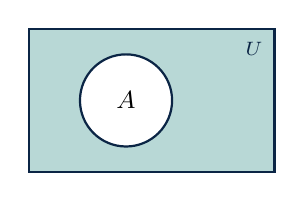
\begin{tikzpicture}[scale=0.65]
  \draw[thick, draw=navy, fill=teal!30] (-1.9,-1.4) rectangle (2.9,1.4);
  \node[navy, font=\bfseries\scriptsize] at (2.5,1.0) {$U$};
  \fill[white] (0,0) circle (0.9);
  \draw[thick, draw=navy] (0,0) circle (0.9);
  \node[font=\bfseries\small] at (0,0) {$A$};
\end{tikzpicture} &
% 5. Symmetric Difference
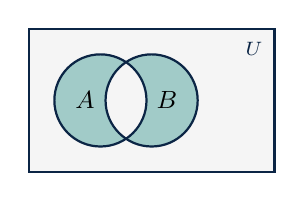
\begin{tikzpicture}[scale=0.65]
  \draw[thick, draw=navy, fill=gray!8] (-1.9,-1.4) rectangle (2.9,1.4);
  \node[navy, font=\bfseries\scriptsize] at (2.5,1.0) {$U$};
  \fill[teal!40] (-0.5,0) circle (0.9);
  \fill[teal!40] (0.5,0) circle (0.9);
  \begin{scope}
    \clip (-0.5,0) circle (0.9);
    \fill[gray!8] (0.5,0) circle (0.9);
  \end{scope}
  \draw[thick, draw=navy] (-0.5,0) circle (0.9);
  \draw[thick, draw=navy] (0.5,0) circle (0.9);
  \node[font=\bfseries\small] at (-0.8,0) {$A$};
  \node[font=\bfseries\small] at (0.8,0) {$B$};
\end{tikzpicture} &
% 6. Disjoint Sets
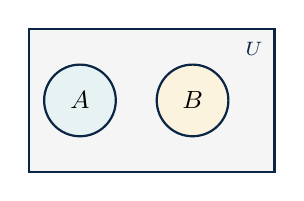
\begin{tikzpicture}[scale=0.65]
  \draw[thick, draw=navy, fill=gray!8] (-1.9,-1.4) rectangle (2.9,1.4);
  \node[navy, font=\bfseries\scriptsize] at (2.5,1.0) {$U$};
  \draw[thick, draw=navy, fill=lightteal] (-0.9,0) circle (0.7);
  \draw[thick, draw=navy, fill=lightgold] (1.3,0) circle (0.7);
  \node[font=\bfseries\small] at (-0.9,0) {$A$};
  \node[font=\bfseries\small] at (1.3,0) {$B$};
\end{tikzpicture} \\
\textbf{(d) Complement: } $\overline{A}$ & \textbf{(e) Symm. Difference: } $A \oplus B$ & \textbf{(f) Disjoint Sets: } $A \cap B = \emptyset$ \\
\end{tabular}
\end{center}

\subsection{The 5 Core Operations Formalized}
\begin{defbox}[Mathematical Definitions of Set Operations]
\begin{enumerate}
    \item \textbf{Union ($A \cup B$):} Elements belonging to $A$ \textbf{or} $B$ (or both):
    \[
    A \cup B = \{x \mid x \in A \lor x \in B\}
    \]
    \item \textbf{Intersection ($A \cap B$):} Elements belonging to \textbf{both} $A$ and $B$:
    \[
    A \cap B = \{x \mid x \in A \land x \in B\}
    \]
    If $A \cap B = \emptyset$, sets $A$ and $B$ are said to be \textbf{mutually disjoint}.
    \item \textbf{Set Difference / Relative Complement ($A \setminus B$ or $A - B$):} Elements in $A$ that are \textbf{not} in $B$:
    \[
    A \setminus B = \{x \mid x \in A \land x \notin B\} = A \cap \overline{B}
    \]
    \item \textbf{Absolute Complement ($\overline{A}$ or $A^c$):} Elements in the Universal set $\mathcal{U}$ that do not belong to $A$:
    \[
    \overline{A} = \mathcal{U} \setminus A = \{x \in \mathcal{U} \mid x \notin A\}
    \]
    \item \textbf{Symmetric Difference ($A \oplus B$ or $A \ \Delta \ B$):} Elements belonging to $A$ or $B$, but \textbf{not both} (The XOR of Sets):
    \[
    \mathbf{A \oplus B = (A \setminus B) \cup (B \setminus A) = (A \cup B) \setminus (A \cap B)}
    \]
\end{enumerate}
\end{defbox}

\begin{exambox}{[SEC TT-01, CSE (DM), year not printed on paper] \ Elementary Set Operations}
\Qlabel
Let $A = \{1, 2, 3, 4, 5\}$ and $B = \{3, 4, 5, 6, 7\}$. Perform the following operations: (i) $A \cup B$ \ (ii) $A \cap B$ \ (iii) $A - B$ \ (iv) $B - A$. \hfill\textit{[8]}
\tcblower
\Alabel
(i) $A \cup B = \mathbf{\{1,2,3,4,5,6,7\}}$ \quad (ii) $A \cap B = \mathbf{\{3,4,5\}}$ \quad (iii) $A - B = \mathbf{\{1,2\}}$ \quad (iv) $B - A = \mathbf{\{6,7\}}$
\end{exambox}

\begin{exambox}{[SEC Final Examination 2024, CSE 0541 1143] \ Venn Diagram Shading}
\Qlabel
Consider Universal set $U$ and two sets $A$ and $B$. Shade the following sets using a Venn diagram: (i) $A \cap B^{C}$ \ (ii) $(B/A)^{C}$. \hfill\textit{[4]}
\tcblower
\Alabel
\begin{center}
\begin{tabular}{cc}
% Region 1: A \cap B^c
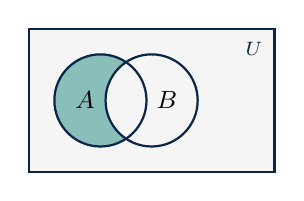
\begin{tikzpicture}[scale=0.65]
  \draw[thick, draw=navy, fill=gray!8] (-1.9,-1.4) rectangle (2.9,1.4);
  \node[navy, font=\bfseries\scriptsize] at (2.5,1.0) {$U$};
  \begin{scope}
    \clip (-0.5,0) circle (0.9);
    \fill[teal!50] (-0.5,0) circle (0.9);
    \fill[gray!8] (0.5,0) circle (0.9);
  \end{scope}
  \draw[thick, draw=navy] (-0.5,0) circle (0.9);
  \draw[thick, draw=navy] (0.5,0) circle (0.9);
  \node[font=\bfseries\small] at (-0.8,0) {$A$};
  \node[font=\bfseries\small] at (0.8,0) {$B$};
\end{tikzpicture} &
% Region 2: (B \setminus A)^c
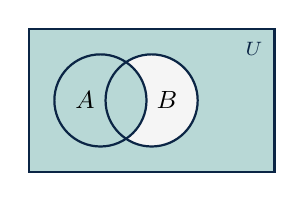
\begin{tikzpicture}[scale=0.65]
  \draw[thick, draw=navy, fill=teal!30] (-1.9,-1.4) rectangle (2.9,1.4);
  \node[navy, font=\bfseries\scriptsize] at (2.5,1.0) {$U$};
  \fill[teal!30] (-0.5,0) circle (0.9);
  \begin{scope}
    \clip (0.5,0) circle (0.9);
    \fill[gray!8] (0.5,0) circle (0.9);
    \fill[teal!30] (-0.5,0) circle (0.9);
  \end{scope}
  \draw[thick, draw=navy] (-0.5,0) circle (0.9);
  \draw[thick, draw=navy] (0.5,0) circle (0.9);
  \node[font=\bfseries\small] at (-0.8,0) {$A$};
  \node[font=\bfseries\small] at (0.8,0) {$B$};
\end{tikzpicture} \\
\textbf{(i) } $A \cap \overline{B} = A \setminus B$ & \textbf{(ii) } $\overline{B \setminus A} = \overline{B} \cup A$
\end{tabular}
\end{center}
(i) By the difference law, $A\cap\overline{B}=A\setminus B$: shaded strictly inside $A$, excluding $A\cap B$. \quad
(ii) Complement of the crescent $B\setminus A$: shaded throughout $U$ except that crescent.
\end{exambox}

% ==============================================================================
% MODULE 6: ALGEBRA OF SETS & DE MORGAN'S LAWS
% ==============================================================================
\section{The Algebra of Sets \& De Morgan’s Laws}

Because set operations are isomorphic to Boolean propositional logic ($\cup \leftrightarrow \lor$, $\cap \leftrightarrow \land$, $\overline{A} \leftrightarrow \neg p$), set algebra obeys an identical set of algebraic laws:

\begin{center}
\renewcommand{\arraystretch}{1.25}
\begin{tabularx}{\textwidth}{l X X}
\toprule
\rowcolor{navy!10} \textbf{Law Name} & \textbf{Union ($\cup$) Form} & \textbf{Intersection ($\cap$) Form} \\
\midrule
\textbf{Identity Laws} & $A \cup \emptyset = A$ & $A \cap \mathcal{U} = A$ \\
\textbf{Domination Laws} & $A \cup \mathcal{U} = \mathcal{U}$ & $A \cap \emptyset = \emptyset$ \\
\textbf{Idempotent Laws} & $A \cup A = A$ & $A \cap A = A$ \\
\textbf{Double Complement} & \multicolumn{2}{c}{$\overline{\overline{A}} = A$} \\
\textbf{Commutative Laws} & $A \cup B = B \cup A$ & $A \cap B = B \cap A$ \\
\textbf{Associative Laws} & $(A \cup B) \cup C = A \cup (B \cup C)$ & $(A \cap B) \cap C = A \cap (B \cap C)$ \\
\textbf{Distributive Laws} & $A \cup (B \cap C) = (A \cup B) \cap (A \cup C)$ & $A \cap (B \cup C) = (A \cap B) \cup (A \cap C)$ \\
\textbf{De Morgan's Laws} & $\mathbf{\overline{A \cup B} = \overline{A} \cap \overline{B}}$ & $\mathbf{\overline{A \cap B} = \overline{A} \cup \overline{B}}$ \\
\textbf{Absorption Laws} & $A \cup (A \cap B) = A$ & $A \cap (A \cup B) = A$ \\
\textbf{Complement Laws} & $A \cup \overline{A} = \mathcal{U}$ & $A \cap \overline{A} = \emptyset$ \\
\bottomrule
\end{tabularx}
\end{center}

\begin{theorembox}[Rigorous Analytical Proof: First De Morgan Law]
\textbf{Theorem:} Prove that $\overline{A \cup B} = \overline{A} \cap \overline{B}$.\\
\textbf{Proof Strategy (Mutual Subset Inclusion):} To prove two sets $X = Y$, we prove $X \subseteq Y$ and $Y \subseteq X$. Equivalently, we use chains of logical equivalences:
\begin{align*}
x \in \overline{A \cup B} &\iff x \notin (A \cup B) && \text{(Definition of complement)} \\
&\iff \neg \big(x \in (A \cup B)\big) && \text{(Definition of $\notin$)} \\
&\iff \neg (x \in A \lor x \in B) && \text{(Definition of union)} \\
&\iff (\neg (x \in A)) \land (\neg (x \in B)) && \text{(De Morgan's Law of Propositional Logic!)} \\
&\iff (x \notin A) \land (x \notin B) && \text{(Definition of $\notin$)} \\
&\iff (x \in \overline{A}) \land (x \in \overline{B}) && \text{(Definition of complement)} \\
&\iff x \in (\overline{A} \cap \overline{B}) && \text{(Definition of intersection)}
\end{align*}
Since each step is a bidirectional logical equivalence ($\iff$), it follows that:
\[
\overline{A \cup B} = \overline{A} \cap \overline{B}. \qquad \blacksquare
\]
\end{theorembox}

\begin{exambox}{[SEC Final Examination 2024, CSE 0541 1143] \ Set Identity Proofs \& Absorption}
\Qlabel
Prove the following using set identities and logical equivalences:
\begin{enumerate}[label=(\roman*)]
    \item $A \cap (A \cap B) = A \cap B$ \quad \textit{(Printed in paper; also proved for $A \cup (A \cap B) = A$)}
    \item $A \cap (A \cup B) = A$ \quad \textit{(Absorption Law)}
\end{enumerate}
\hfill\textit{[05]}
\tcblower
\Alabel
\textbf{Proof of (i):}
By the Associative Law of set intersection:
\[
A \cap (A \cap B) = (A \cap A) \cap B
\]
By the Idempotent Law ($A \cap A = A$):
\[
(A \cap A) \cap B = \mathbf{A \cap B}. \qquad \blacksquare
\]
\textit{Note on Examination Variant ($A \cup (A \cap B) = A$):}
\begin{align*}
x \in A \cup (A \cap B) &\iff x \in A \lor (x \in A \land x \in B) \\
&\iff (x \in A \lor x \in A) \land (x \in A \lor x \in B) && \text{(Distributivity)} \\
&\iff x \in A \land (x \in A \lor x \in B) \iff x \in A. && \text{(Absorption in Logic)}
\end{align*}

\medskip
\textbf{Proof of (ii) $A \cap (A \cup B) = A$ (Absorption Law):}
We establish equality via mutual subset inclusion:
\begin{enumerate}
    \item \textbf{Show $A \cap (A \cup B) \subseteq A$:}
    Let $x \in A \cap (A \cup B)$. By definition of intersection, $x \in A$ and $x \in (A \cup B)$. In particular, $x \in A$. Therefore, $A \cap (A \cup B) \subseteq A$.
    \item \textbf{Show $A \subseteq A \cap (A \cup B)$:}
    Let $x \in A$. Then certainly $x \in A \cup B$ (by definition of union). Since $x \in A$ and $x \in A \cup B$, it follows that $x \in A \cap (A \cup B)$. Therefore, $A \subseteq A \cap (A \cup B)$.
\end{enumerate}
Since both inclusions hold, $\mathbf{A \cap (A \cup B) = A}$. $\blacksquare$
\end{exambox}

% ==============================================================================
% MODULE 7: PRINCIPLE OF INCLUSION-EXCLUSION
% ==============================================================================
\section{The Principle of Inclusion-Exclusion (PIE)}

When counting elements in overlapping sets, simply adding $|A| + |B|$ double-counts the common intersection. We must subtract the overlap to restore balance:

\subsection{PIE for 2 Sets}
\[
\mathbf{|A \cup B| = |A| + |B| - |A \cap B|}
\]

\begin{exambox}{[SEC TT-01, CSE 103, 2022] \ Two-Set Overlap: Class Attendance Lists}
\Qlabel
List $A$ contains the 30 students in a mathematics class, and list $B$ contains the 35 students in an English class; 20 names appear on both lists. Find the number of students: (a) only on list $A$, (b) only on list $B$, (c) on list $A$ or $B$ (or both), (d) on exactly one list. \hfill\textit{[5]}
\tcblower
\Alabel
$|A\setminus B| = 30-20 = \mathbf{10}$ \quad $|B\setminus A| = 35-20 = \mathbf{15}$ \quad $|A\cup B| = 30+35-20 = \mathbf{45}$ \quad $|A \oplus B| = 10+15 = \mathbf{25}$
\end{exambox}

\begin{exambox}{[SEC Final Examination 2022, CSE 103] \ Venn Diagram Survey of Requirements}
\Qlabel
Each student in Liberal Arts has a mathematics requirement $A$ and a science requirement $B$. A poll of 140 sophomore students shows: 60 completed $A$, 45 completed $B$, 20 completed both. Use a Venn diagram to find the number of students who completed: (i) at least one of $A$ and $B$; (ii) exactly one of $A$ or $B$; (iii) neither $A$ nor $B$. \hfill\textit{[1$\times$3]}
\tcblower
\Alabel
\begin{center}
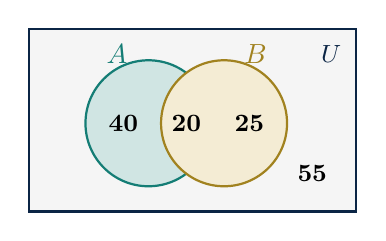
\begin{tikzpicture}[scale=0.8]
  \draw[thick, draw=navy, fill=gray!8] (-2.5,-1.4) rectangle (2.7,1.5);
  \node[navy, font=\bfseries\small] at (2.3,1.1) {$U$};
  \draw[thick, draw=teal, fill=teal!20] (-0.6,0) circle (1.0);
  \draw[thick, draw=gold!80!black, fill=gold!20] (0.6,0) circle (1.0);
  \node[font=\bfseries\small] at (-1.0,0) {40};
  \node[font=\bfseries\small] at (0,0) {20};
  \node[font=\bfseries\small] at (1.0,0) {25};
  \node[font=\bfseries\small] at (2.0,-0.8) {55};
  \node[font=\bfseries\color{teal}] at (-1.1,1.1) {$A$};
  \node[font=\bfseries\color{gold!80!black}] at (1.1,1.1) {$B$};
\end{tikzpicture}
\end{center}
(i) $|A \cup B| = 60+45-20 = \mathbf{85}$. \quad
(ii) $|A\setminus B|+|B\setminus A| = 40+25 = \mathbf{65}$. \quad
(iii) $|U|-|A\cup B| = 140-85 = \mathbf{55}$.
\end{exambox}

\newpage
\subsection{PIE for 3 Sets}
For three arbitrary finite sets $A$, $B$, and $C$:
\[
\mathbf{|A \cup B \cup C| = |A| + |B| + |C| - |A \cap B| - |B \cap C| - |A \cap C| + |A \cap B \cap C|}
\]

\begin{center}
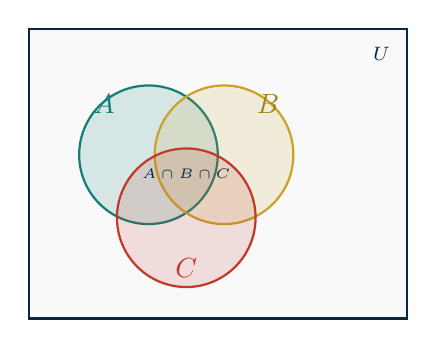
\begin{tikzpicture}[scale=0.8]
  \draw[thick, draw=navy, fill=gray!5] (-2.5,-2.2) rectangle (3.5,2.4);
  \node[navy, font=\bfseries\scriptsize] at (3.1,2.0) {$U$};
  
  \draw[thick, draw=teal, fill=teal, fill opacity=0.15] (-0.6, 0.4) circle (1.1);
  \draw[thick, draw=gold, fill=gold, fill opacity=0.15] (0.6, 0.4) circle (1.1);
  \draw[thick, draw=coral, fill=coral, fill opacity=0.15] (0, -0.6) circle (1.1);
  
  \node[font=\bfseries\color{teal}] at (-1.3, 1.2) {$A$};
  \node[font=\bfseries\color{gold!80!black}] at (1.3, 1.2) {$B$};
  \node[font=\bfseries\color{coral}] at (0, -1.4) {$C$};
  
  \node[font=\tiny\bfseries\color{navy}] at (0, 0.1) {$A \cap B \cap C$};
\end{tikzpicture}\\[3pt]
{\small\textit{\color{navy}\textbf{Figure 3:} The 3-set overlapping geometry of the Inclusion-Exclusion Principle.}}
\end{center}

\begin{exambox}{[SEC Final Examination 2024, CSE 0541 1143] \ Three-Set Language Enrollment}
\Qlabel
In a class of 80 students, 50 know English ($E$), 55 know French ($F$), 46 know German ($G$). 37 know English and French, 28 know French and German, 21 know English and German. 7 know none of the three languages. How many students know all three languages? \hfill\textit{[04]}
\tcblower
\Alabel
Knowing at least one: $|E\cup F\cup G| = 80-7 = 73$. By PIE:
\[
73 = 50+55+46-(37+28+21)+|E\cap F\cap G| = 65 + |E\cap F\cap G| \implies \mathbf{|E\cap F\cap G| = 8}
\]
\textbf{8 students} know all three languages.
\end{exambox}

\begin{exambox}{[SEC Final Examination 2024, CSE 0541 1143] \ Three-Set Subject Preferences}
\Qlabel
Out of 100 students, 50 like English ($E$), 35 like Science ($S$), 29 like Math ($M$). 6 like Math and English, 8 like English and Science, 6 like Science and Math. Only 5 like all three subjects. How many students don't like any of these subjects? (Use Venn diagram) \hfill\textit{[04]}
\tcblower
\Alabel
\[
|E \cup S \cup M| = 50+35+29-(8+6+6)+5 = 114-20+5 = \mathbf{99}
\]
Students liking none: $|U|-|E\cup S\cup M| = 100-99 = \mathbf{1 \text{ student}}$.
\end{exambox}

% ==============================================================================
% MODULE 8: FUNCTIONS (MAPPINGS, INJECTIONS, SURJECTIONS & BIJECTIONS)
% ==============================================================================
\newpage
\section{\texorpdfstring{$\bigstar$ }{*}Functions: Definitions, Types, Inverses \& Compositions}
\noindent{\footnotesize\color{teal}\textbf{$\bigstar$ SEC Syllabus Core Topic:} \textit{Functions, Domain/Codomain/Range, Injections, Surjections, Bijections, Inverses, Compositions, Floor/Ceiling}}\\[4pt]

A \textbf{function} (or \textit{mapping}) is a foundational mathematical construct underpinning functional programming, algorithmic analysis, hashing, and cryptography. Set-theoretically, a function is a constrained binary relation.

\subsection{Formal Definition of a Function}

\begin{defbox}[Formal Definition of a Function]
Let $A$ and $B$ be non-empty sets. A \textbf{function} $f$ from $A$ to $B$, denoted:
\[
f: A \to B
\]
is a relation $f \subseteq A \times B$ that assigns to \textbf{each} element $a \in A$ \textbf{exactly one} element $b \in B$. We write $f(a) = b$, where:
\begin{itemize}
    \item $A$ is the \textbf{Domain} of $f$, denoted $\operatorname{Dom}(f) = A$.
    \item $B$ is the \textbf{Codomain} of $f$, denoted $\operatorname{Codom}(f) = B$.
    \item $b$ is the \textbf{image} of $a$ under $f$, and $a$ is a \textbf{preimage} of $b$.
    \item The \textbf{Range} (or \textit{Image} of $A$) is the set of all actual outputs:
    \[
    \operatorname{Range}(f) = f(A) = \{f(a) \mid a \in A\} = \{b \in B \mid \exists a \in A \text{ such that } f(a) = b\}
    \]
\end{itemize}
\end{defbox}

\begin{center}
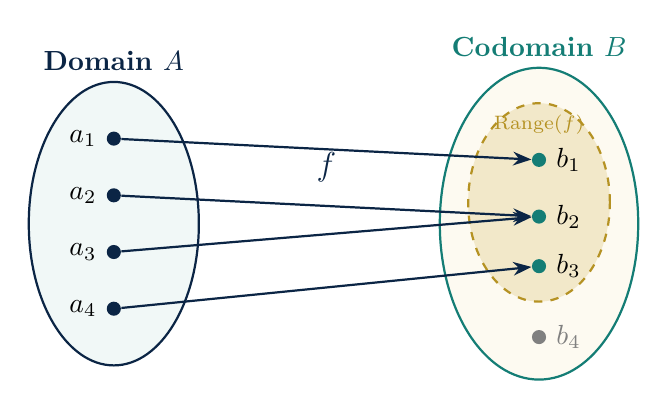
\begin{tikzpicture}[scale=0.9, >=Stealth]
  % Domain A
  \draw[thick, draw=navy, fill=lightteal!60] (-3, 0) ellipse (1.2 and 2.0);
  \node[navy, font=\bfseries\normalsize] at (-3, 2.3) {Domain $A$};
  \node[circle, fill=navy, inner sep=1.8pt, label=left:{$a_1$}] (a1) at (-3, 1.2) {};
  \node[circle, fill=navy, inner sep=1.8pt, label=left:{$a_2$}] (a2) at (-3, 0.4) {};
  \node[circle, fill=navy, inner sep=1.8pt, label=left:{$a_3$}] (a3) at (-3, -0.4) {};
  \node[circle, fill=navy, inner sep=1.8pt, label=left:{$a_4$}] (a4) at (-3, -1.2) {};

  % Codomain B
  \draw[thick, draw=teal, fill=lightgold!40] (3, 0) ellipse (1.4 and 2.2);
  \node[teal, font=\bfseries\normalsize] at (3, 2.5) {Codomain $B$};
  
  % Range subset
  \draw[thick, dashed, draw=gold!90!black, fill=gold!25] (3, 0.3) ellipse (1.0 and 1.4);
  \node[gold!90!black, font=\bfseries\scriptsize] at (3, 1.4) {$\operatorname{Range}(f)$};
  
  \node[circle, fill=teal, inner sep=1.8pt, label=right:{$b_1$}] (b1) at (3, 0.9) {};
  \node[circle, fill=teal, inner sep=1.8pt, label=right:{$b_2$}] (b2) at (3, 0.1) {};
  \node[circle, fill=teal, inner sep=1.8pt, label=right:{$b_3$}] (b3) at (3, -0.6) {};
  \node[circle, fill=gray, inner sep=1.8pt, label=right:{\color{gray}$b_4$}] (b4) at (3, -1.6) {};

  % Arrows
  \draw[->, thick, navy] (a1) -- (b1);
  \draw[->, thick, navy] (a2) -- (b2);
  \draw[->, thick, navy] (a3) -- (b2);
  \draw[->, thick, navy] (a4) -- (b3);

  \node[navy, font=\bfseries\large] at (0, 0.8) {$f$};
\end{tikzpicture}\\[3pt]
{\small\textit{\color{navy}\textbf{Figure 4:} Anatomy of a function: Domain $A$, Codomain $B$, and Range $f(A) \subseteq B$. Note $b_4 \notin \operatorname{Range}(f)$.}}
\end{center}

\begin{warningbox}[The Universal Beginner Trap: Codomain vs. Range]
Never confuse the \textbf{Codomain} with the \textbf{Range}!
\begin{itemize}
    \item The \textbf{Codomain} is the target set specified in the function declaration ($B$ in $f: A \to B$).
    \item The \textbf{Range} is the set of elements in $B$ that are actually hit by at least one $a \in A$.
    \item In general, $\mathbf{\operatorname{Range}(f) \subseteq \operatorname{Codomain}(f)}$. They are equal \textbf{if and only if} $f$ is \textbf{surjective} (onto).
\end{itemize}
\end{warningbox}

\begin{theorembox}[Equality Criterion for Two Functions]
Two functions $f$ and $g$ are \textbf{equal} ($f = g$) if and only if:
\begin{enumerate}
    \item $\operatorname{Dom}(f) = \operatorname{Dom}(g)$,
    \item $\operatorname{Codom}(f) = \operatorname{Codom}(g)$, and
    \item $f(x) = g(x)$ for all $x \in \operatorname{Dom}(f)$.
\end{enumerate}
\textit{Example:} $f: \mathbb{R} \to \mathbb{R}$ where $f(x) = x$ and $g: \mathbb{Z} \to \mathbb{R}$ where $g(x) = x$ are \textbf{NOT equal} because $\operatorname{Dom}(f) \neq \operatorname{Dom}(g)$.
\end{theorembox}

\subsection{One-to-One Functions (Injections)}

\begin{defbox}[Injective / One-to-One Function]
A function $f: A \to B$ is \textbf{one-to-one} (or an \textbf{injection}) if and only if distinct elements in the domain have distinct images in the codomain.
\[
\mathbf{\forall x_1, x_2 \in A, \quad f(x_1) = f(x_2) \implies x_1 = x_2}
\]
Equivalently, by contraposition:
\[
\mathbf{\forall x_1, x_2 \in A, \quad x_1 \neq x_2 \implies f(x_1) \neq f(x_2)}
\]
\end{defbox}

\begin{center}
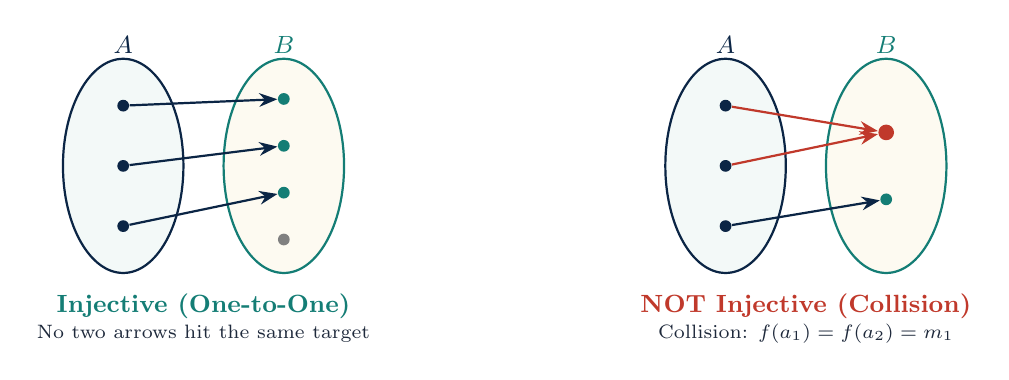
\begin{tikzpicture}[scale=0.85, >=Stealth]
  % Injective Diagram
  \begin{scope}[xshift=-4.5cm]
    \draw[thick, draw=navy, fill=lightteal!50] (-1.2,0) ellipse (0.9 and 1.6);
    \draw[thick, draw=teal, fill=lightgold!40] (1.2,0) ellipse (0.9 and 1.6);
    \node[navy, font=\bfseries\small] at (-1.2, 1.8) {$A$};
    \node[teal, font=\bfseries\small] at (1.2, 1.8) {$B$};
    
    \node[circle, fill=navy, inner sep=1.5pt] (i1) at (-1.2, 0.9) {};
    \node[circle, fill=navy, inner sep=1.5pt] (i2) at (-1.2, 0) {};
    \node[circle, fill=navy, inner sep=1.5pt] (i3) at (-1.2, -0.9) {};
    
    \node[circle, fill=teal, inner sep=1.5pt] (j1) at (1.2, 1.0) {};
    \node[circle, fill=teal, inner sep=1.5pt] (j2) at (1.2, 0.3) {};
    \node[circle, fill=teal, inner sep=1.5pt] (j3) at (1.2, -0.4) {};
    \node[circle, fill=gray, inner sep=1.5pt] (j4) at (1.2, -1.1) {};
    
    \draw[->, thick, navy] (i1) -- (j1);
    \draw[->, thick, navy] (i2) -- (j2);
    \draw[->, thick, navy] (i3) -- (j3);
    \node[font=\bfseries\small\color{teal}] at (0, -2.1) {Injective (One-to-One)};
    \node[font=\scriptsize\color{darkslate}] at (0, -2.5) {No two arrows hit the same target};
  \end{scope}

  % Not Injective Diagram
  \begin{scope}[xshift=4.5cm]
    \draw[thick, draw=navy, fill=lightteal!50] (-1.2,0) ellipse (0.9 and 1.6);
    \draw[thick, draw=teal, fill=lightgold!40] (1.2,0) ellipse (0.9 and 1.6);
    \node[navy, font=\bfseries\small] at (-1.2, 1.8) {$A$};
    \node[teal, font=\bfseries\small] at (1.2, 1.8) {$B$};
    
    \node[circle, fill=navy, inner sep=1.5pt] (k1) at (-1.2, 0.9) {};
    \node[circle, fill=navy, inner sep=1.5pt] (k2) at (-1.2, 0) {};
    \node[circle, fill=navy, inner sep=1.5pt] (k3) at (-1.2, -0.9) {};
    
    \node[circle, fill=coral, inner sep=2.0pt] (m1) at (1.2, 0.5) {};
    \node[circle, fill=teal, inner sep=1.5pt] (m2) at (1.2, -0.5) {};
    
    \draw[->, thick, coral] (k1) -- (m1);
    \draw[->, thick, coral] (k2) -- (m1);
    \draw[->, thick, navy] (k3) -- (m2);
    \node[font=\bfseries\small\color{coral}] at (0, -2.1) {NOT Injective (Collision)};
    \node[font=\scriptsize\color{darkslate}] at (0, -2.5) {Collision: $f(a_1) = f(a_2) = m_1$};
  \end{scope}
\end{tikzpicture}
\end{center}

\begin{examplebox}[Analytical Proofs: Proving vs. Disproving Injectivity]
\begin{enumerate}
    \item \textbf{Prove $f: \mathbb{R} \to \mathbb{R}$ defined by $f(x) = 4x - 7$ is Injective:}\\
    \textit{Proof:} Assume $f(x_1) = f(x_2)$. Then:
    \[
    4x_1 - 7 = 4x_2 - 7 \implies 4x_1 = 4x_2 \implies x_1 = x_2.
    \]
    Since $f(x_1) = f(x_2) \implies x_1 = x_2$, $f$ is strictly injective. $\blacksquare$

    \item \textbf{Disprove that $g: \mathbb{R} \to \mathbb{R}$ defined by $g(x) = x^2$ is Injective:}\\
    \textit{Refutation (Counter-example Method):} To disprove $\forall x_1, x_2 (g(x_1)=g(x_2) \implies x_1=x_2)$, find one explicit pair where $x_1 \neq x_2$ but $g(x_1) = g(x_2)$.\\
    Choose $x_1 = 2$ and $x_2 = -2$. Notice $x_1 \neq x_2$, but:
    \[
    g(2) = 2^2 = 4 \quad \text{and} \quad g(-2) = (-2)^2 = 4 \implies g(2) = g(-2).
    \]
    Therefore, $g$ is \textbf{not injective}.
\end{enumerate}
\end{examplebox}

\subsection{Onto Functions (Surjections)}

\begin{defbox}[Surjective / Onto Function]
A function $f: A \to B$ is \textbf{onto} (or a \textbf{surjection}) if and only if every element in the codomain $B$ is the image of at least one element in the domain $A$:
\[
\mathbf{\forall y \in B, \quad \exists x \in A \quad \text{such that} \quad f(x) = y}
\]
Equivalently:
\[
\mathbf{\operatorname{Range}(f) = \operatorname{Codomain}(f) = B}
\]
\end{defbox}

\begin{center}
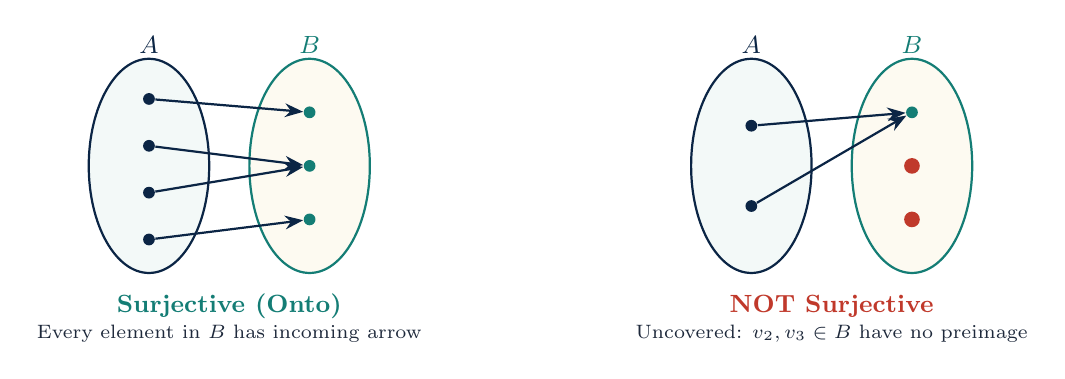
\begin{tikzpicture}[scale=0.85, >=Stealth]
  % Surjective Diagram
  \begin{scope}[xshift=-4.5cm]
    \draw[thick, draw=navy, fill=lightteal!50] (-1.2,0) ellipse (0.9 and 1.6);
    \draw[thick, draw=teal, fill=lightgold!40] (1.2,0) ellipse (0.9 and 1.6);
    \node[navy, font=\bfseries\small] at (-1.2, 1.8) {$A$};
    \node[teal, font=\bfseries\small] at (1.2, 1.8) {$B$};
    
    \node[circle, fill=navy, inner sep=1.5pt] (s1) at (-1.2, 1.0) {};
    \node[circle, fill=navy, inner sep=1.5pt] (s2) at (-1.2, 0.3) {};
    \node[circle, fill=navy, inner sep=1.5pt] (s3) at (-1.2, -0.4) {};
    \node[circle, fill=navy, inner sep=1.5pt] (s4) at (-1.2, -1.1) {};
    
    \node[circle, fill=teal, inner sep=1.5pt] (t1) at (1.2, 0.8) {};
    \node[circle, fill=teal, inner sep=1.5pt] (t2) at (1.2, 0) {};
    \node[circle, fill=teal, inner sep=1.5pt] (t3) at (1.2, -0.8) {};
    
    \draw[->, thick, navy] (s1) -- (t1);
    \draw[->, thick, navy] (s2) -- (t2);
    \draw[->, thick, navy] (s3) -- (t2);
    \draw[->, thick, navy] (s4) -- (t3);
    \node[font=\bfseries\small\color{teal}] at (0, -2.1) {Surjective (Onto)};
    \node[font=\scriptsize\color{darkslate}] at (0, -2.5) {Every element in $B$ has incoming arrow};
  \end{scope}

  % Not Surjective Diagram
  \begin{scope}[xshift=4.5cm]
    \draw[thick, draw=navy, fill=lightteal!50] (-1.2,0) ellipse (0.9 and 1.6);
    \draw[thick, draw=teal, fill=lightgold!40] (1.2,0) ellipse (0.9 and 1.6);
    \node[navy, font=\bfseries\small] at (-1.2, 1.8) {$A$};
    \node[teal, font=\bfseries\small] at (1.2, 1.8) {$B$};
    
    \node[circle, fill=navy, inner sep=1.5pt] (u1) at (-1.2, 0.6) {};
    \node[circle, fill=navy, inner sep=1.5pt] (u2) at (-1.2, -0.6) {};
    
    \node[circle, fill=teal, inner sep=1.5pt] (v1) at (1.2, 0.8) {};
    \node[circle, fill=coral, inner sep=2.0pt] (v2) at (1.2, 0) {};
    \node[circle, fill=coral, inner sep=2.0pt] (v3) at (1.2, -0.8) {};
    
    \draw[->, thick, navy] (u1) -- (v1);
    \draw[->, thick, navy] (u2) -- (v1);
    \node[font=\bfseries\small\color{coral}] at (0, -2.1) {NOT Surjective};
    \node[font=\scriptsize\color{darkslate}] at (0, -2.5) {Uncovered: $v_2, v_3 \in B$ have no preimage};
  \end{scope}
\end{tikzpicture}
\end{center}

\begin{examplebox}[Analytical Proofs: Proving vs. Disproving Surjectivity]
\begin{enumerate}
    \item \textbf{Prove $f: \mathbb{R} \to \mathbb{R}$ with $f(x) = 3x - 5$ is Surjective:}\\
    \textit{Proof Strategy (Finding Preimage):} Let $y \in \mathbb{R}$ be an arbitrary element in the codomain. We must find $x \in \mathbb{R}$ such that $f(x) = y$:
    \[
    y = 3x - 5 \iff 3x = y + 5 \iff x = \frac{y + 5}{3}
    \]
    Since $y \in \mathbb{R}$, $x = \frac{y+5}{3}$ is a well-defined real number ($x \in \mathbb{R}$). Checking:
    \[
    f\left(\frac{y+5}{3}\right) = 3\left(\frac{y+5}{3}\right) - 5 = (y + 5) - 5 = y.
    \]
    Hence, every $y \in \mathbb{R}$ has a valid preimage in $\mathbb{R}$. $f$ is surjective. $\blacksquare$

    \item \textbf{Disprove that $g: \mathbb{Z} \to \mathbb{Z}$ with $g(x) = 2x$ is Surjective:}\\
    \textit{Refutation:} The codomain is $\mathbb{Z}$. Consider $y = 3 \in \mathbb{Z}$. If $g(x) = 3$, then $2x = 3 \implies x = 1.5 \notin \mathbb{Z}$. Since the odd integer $3$ has no preimage in the domain $\mathbb{Z}$, $g$ is \textbf{not surjective}.
\end{enumerate}
\end{examplebox}

\subsection{One-to-One Correspondences (Bijections)}

\begin{defbox}[Bijective Function / One-to-One Correspondence]
A function $f: A \to B$ is a \textbf{bijection} (or a \textbf{one-to-one correspondence}) if and only if it is \textbf{both injective and surjective}.
\[
\mathbf{f \text{ is Bijective}} \iff (\mathbf{f \text{ is Injective}} \ \land \ \mathbf{f \text{ is Surjective}})
\]
\end{defbox}

\begin{center}
\renewcommand{\arraystretch}{1.2}
\begin{tabularx}{\linewidth}{@{}l X X@{}}
\toprule
\rowcolor{navy!15}
\textbf{\color{navy}Classification} & \textbf{\color{navy}Geometric / Relational Meaning} & \textbf{\color{navy}Cardinality Constraint (Finite Sets)} \\
\midrule
\textbf{Injective Only} & Each $b \in B$ receives at most $1$ arrow. & $|A| \le |B|$ \\
\textbf{Surjective Only} & Each $b \in B$ receives at least $1$ arrow. & $|A| \ge |B|$ \\
\rowcolor{lightteal!60}
\textbf{Bijective (Both)} & Each $b \in B$ receives \textbf{exactly 1} arrow. & $\mathbf{|A| = |B|}$ \\
\textbf{Neither} & Collisions exist AND some $b \in B$ are missed. & No cardinality constraint \\
\bottomrule
\end{tabularx}
\end{center}

\subsection{Inverse Functions (\texorpdfstring{$f^{-1}$}{f\textasciicircum-1})}

\begin{defbox}[Inverse Function Definition]
Let $f: A \to B$ be a \textbf{bijective} function. The \textbf{inverse function} of $f$, denoted $f^{-1}: B \to A$, assigns to each element $b \in B$ the unique element $a \in A$ such that $f(a) = b$:
\[
\mathbf{f^{-1}(b) = a \iff f(a) = b}
\]
\end{defbox}

\begin{theorembox}[Invertibility Criterion Theorem]
A function $f: A \to B$ is \textbf{invertible} if and only if it is a \textbf{bijection}.
\begin{itemize}
    \item If $f$ is \textit{not injective}, two distinct domain elements $a_1 \neq a_2$ map to the same $b$. Then $f^{-1}(b)$ would have to return multiple values ($\{a_1, a_2\}$), violating the single-valued definition of a function.
    \item If $f$ is \textit{not surjective}, some $b \in B$ has no preimage. Then $f^{-1}(b)$ would be undefined, violating the requirement that a function must map every element of its domain.
\end{itemize}
\end{theorembox}

\begin{warningbox}[Notation Alert: Inverse Function vs. Reciprocal]
Do not confuse $f^{-1}(x)$ with the algebraic reciprocal $\frac{1}{f(x)}$!
\[
f^{-1}(x) \ \neq \ (f(x))^{-1} = \frac{1}{f(x)}
\]
$f^{-1}$ denotes the \textbf{functional inverse}, whereas $\frac{1}{f(x)}$ is the \textbf{multiplicative inverse} of the numerical output.
\end{warningbox}

\begin{examplebox}[Algorithmic Procedure to Find an Inverse Function]
\textbf{Task:} Let $f: \mathbb{R}\setminus\{2\} \to \mathbb{R}\setminus\{1\}$ defined by $f(x) = \frac{x + 3}{x - 2}$. Find $f^{-1}(x)$.
\begin{enumerate}
    \item \textbf{Step 1: Set $y = f(x)$:}
    \[
    y = \frac{x + 3}{x - 2}
    \]
    \item \textbf{Step 2: Solve algebraically for $x$ in terms of $y$:}
    \[
    y(x - 2) = x + 3 \implies xy - 2y = x + 3 \implies xy - x = 2y + 3 \implies x(y - 1) = 2y + 3
    \]
    \[
    x = \frac{2y + 3}{y - 1} \qquad (\text{defined since } y \neq 1)
    \]
    \item \textbf{Step 3: Interchange variables to express $f^{-1}(x)$:}
    \[
    \mathbf{f^{-1}(x) = \frac{2x + 3}{x - 1}}
    \]
    \item \textbf{Step 4: Verification ($f(f^{-1}(x)) = x$):}
    \[
    f(f^{-1}(x)) = \frac{\frac{2x+3}{x-1} + 3}{\frac{2x+3}{x-1} - 2} = \frac{\frac{2x+3+3x-3}{x-1}}{\frac{2x+3-2x+2}{x-1}} = \frac{5x}{5} = x. \quad \checkmark
    \]
\end{enumerate}
\end{examplebox}

\subsection{Composition of Functions (\texorpdfstring{$f \circ g$}{f o g})}

\begin{defbox}[Composition of Functions]
Let $g: A \to B$ and $f: B \to C$. The \textbf{composition} of $f$ and $g$, denoted by:
\[
\mathbf{f \circ g}: A \to C
\]
is defined for all $x \in A$ by:
\[
\mathbf{(f \circ g)(x) = f\big(g(x)\big)}
\]
\textit{Note the evaluation order:} $g$ operates first on $x$, and then $f$ operates on the resulting value $g(x)$.
\end{defbox}

\begin{center}
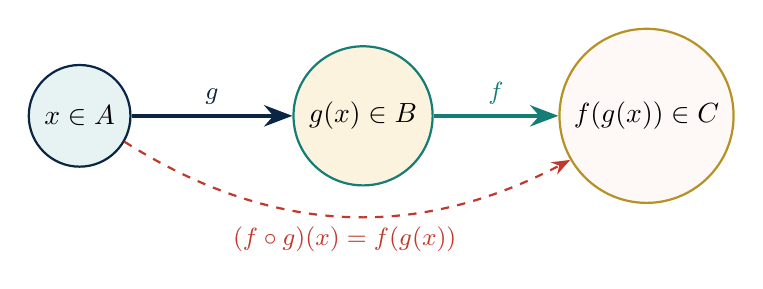
\begin{tikzpicture}[scale=0.9, >=Stealth]
  \node[circle, draw=navy, fill=lightteal, thick, inner sep=4pt] (A) at (0, 0) {$x \in A$};
  \node[circle, draw=teal, fill=lightgold, thick, inner sep=4pt] (B) at (4, 0) {$g(x) \in B$};
  \node[circle, draw=gold!90!black, fill=lightcoral!40, thick, inner sep=4pt] (C) at (8, 0) {$f(g(x)) \in C$};
  
  \draw[->, ultra thick, navy] (A) -- node[above, font=\bfseries\small] {$g$} (B);
  \draw[->, ultra thick, teal] (B) -- node[above, font=\bfseries\small] {$f$} (C);
  
  \draw[->, thick, dashed, coral] (A) to[bend right=30] node[below, font=\bfseries\small] {$(f \circ g)(x) = f(g(x))$} (C);
\end{tikzpicture}
\end{center}

\begin{theorembox}[Algebraic Properties of Composition]
\begin{enumerate}
    \item \textbf{Associativity:} If $h: A \to B$, $g: B \to C$, and $f: C \to D$, then:
    \[
    f \circ (g \circ h) = (f \circ g) \circ h
    \]
    \item \textbf{Non-Commutativity (Crucial!):} In general:
    \[
    \mathbf{f \circ g \ \neq \ g \circ f}
    \]
    \textit{Counterexample:} Let $f(x) = 2x$ and $g(x) = x + 1$.
    \[
    (f \circ g)(x) = f(x+1) = 2(x+1) = 2x + 2, \qquad (g \circ f)(x) = g(2x) = 2x + 1 \implies f \circ g \neq g \circ f.
    \]
    \item \textbf{Identity with Inverse:} If $f: A \to B$ is a bijection, then:
    \[
    f^{-1} \circ f = \operatorname{id}_A \quad \text{and} \quad f \circ f^{-1} = \operatorname{id}_B
    \]
    \item \textbf{Preservation of Injectivity / Surjectivity / Bijectivity:}
    \begin{itemize}
        \item If $f$ and $g$ are both injective, then $f \circ g$ is \textbf{injective}.
        \item If $f$ and $g$ are both surjective, then $f \circ g$ is \textbf{surjective}.
        \item If $f$ and $g$ are both bijective, then $f \circ g$ is \textbf{bijective}, and $(f \circ g)^{-1} = g^{-1} \circ f^{-1}$.
    \end{itemize}
\end{enumerate}
\end{theorembox}

\subsection{Essential Special Functions in Computer Science}

\begin{defbox}[Floor and Ceiling Functions]
\begin{itemize}
    \item The \textbf{Floor function} $\lfloor x \rfloor$ assigns to the real number $x$ the largest integer that is less than or equal to $x$:
    \[
    \lfloor x \rfloor = n \iff n \le x < n + 1, \quad n \in \mathbb{Z}
    \]
    \item The \textbf{Ceiling function} $\lceil x \rceil$ assigns to the real number $x$ the smallest integer that is greater than or equal to $x$:
    \[
    \lceil x \rceil = n \iff n - 1 < x \le n, \quad n \in \mathbb{Z}
    \]
\end{itemize}
\end{defbox}

\begin{notebox}[Useful Mathematical Properties of Floor and Ceiling]
\renewcommand{\arraystretch}{1.2}
\begin{tabularx}{\linewidth}{@{}l X l@{}}
\toprule
\textbf{\color{navy}Property Name} & \textbf{\color{navy}Mathematical Formula} & \textbf{\color{navy}Context ($n \in \mathbb{Z}, x \in \mathbb{R}$)} \\
\midrule
\textbf{Integer Identity} & $\lfloor x \rfloor = x \iff x \in \mathbb{Z} \iff \lceil x \rceil = x$ & Exact integer equality \\
\textbf{Bounds} & $x - 1 < \lfloor x \rfloor \le x \le \lceil x \rceil < x + 1$ & Tight squeeze inequalities \\
\textbf{Integer Shift} & $\lfloor x + n \rfloor = \lfloor x \rfloor + n, \quad \lceil x + n \rceil = \lceil x \rceil + n$ & Pulling integers outside \\
\textbf{Negative Symmetry} & $\lfloor -x \rfloor = -\lceil x \rceil, \quad \lceil -x \rceil = -\lfloor x \rfloor$ & Sign flipping inversion \\
\textbf{Duplication Formula} & $\mathbf{\lfloor 2x \rfloor = \lfloor x \rfloor + \lfloor x + \frac{1}{2} \rfloor}$ & Hermite's Identity ($k=2$) \\
\bottomrule
\end{tabularx}
\end{notebox}

\begin{examplebox}[CS Algorithmic Applications of Floor \& Ceiling]
\begin{itemize}
    \item \textbf{Binary Bit-Length of an Integer $n$:} The number of bits required to represent a positive integer $n$ in binary is:
    \[
    b(n) = \lfloor \log_2 n \rfloor + 1
    \]
    \textit{Example:} For $n = 25$, $\log_2(25) \approx 4.6438 \implies \lfloor 4.6438 \rfloor + 1 = 4 + 1 = \mathbf{5 \text{ bits}}$ ($25_{10} = 11001_2$).
    \item \textbf{Height of a Complete Binary Tree:} A complete binary tree with $n$ nodes has height:
    \[
    h = \lceil \log_2(n + 1) \rceil - 1
    \]
    \item \textbf{Page Allocation in Memory / Pagination:} Dividing $N$ data records into pages of size $S$ requires:
    \[
    \text{Pages} = \left\lceil \frac{N}{S} \right\rceil
    \]
\end{itemize}
\end{examplebox}

\subsection{Past SEC Examination Questions on Functions}

\begin{exambox}{[SEC Final Examination, CSE 0541 1143] \ Injectivity, Surjectivity \& Inverse}
\Qlabel
Let $A = \mathbb{R} \setminus \{2\}$ and $B = \mathbb{R} \setminus \{1\}$. Define $f: A \to B$ by:
\[
f(x) = \frac{x - 3}{x - 2}
\]
(a) Prove that $f$ is bijective. \hfill\textit{[4]}\\
(b) Find the explicit formula for $f^{-1}(x)$ and state its domain. \hfill\textit{[2]}
\tcblower
\Alabel
\textbf{(a) Proof of Bijectivity:}
\begin{enumerate}
    \item \textbf{Injectivity:} Let $x_1, x_2 \in A$ such that $f(x_1) = f(x_2)$:
    \[
    \frac{x_1 - 3}{x_1 - 2} = \frac{x_2 - 3}{x_2 - 2} \implies (x_1 - 3)(x_2 - 2) = (x_2 - 3)(x_1 - 2)
    \]
    Expanding both sides:
    \[
    x_1 x_2 - 2x_1 - 3x_2 + 6 = x_1 x_2 - 2x_2 - 3x_1 + 6
    \]
    Canceling $x_1 x_2 + 6$ from both sides:
    \[
    -2x_1 - 3x_2 = -2x_2 - 3x_1 \implies 3x_1 - 2x_1 = 3x_2 - 2x_2 \implies x_1 = x_2.
    \]
    Thus, $f$ is strictly \textbf{injective}.
    
    \item \textbf{Surjectivity:} Let $y \in B = \mathbb{R} \setminus \{1\}$. We show there exists $x \in A$ such that $f(x) = y$:
    \[
    y = \frac{x - 3}{x - 2} \implies y(x - 2) = x - 3 \implies xy - 2y = x - 3 \implies x(y - 1) = 2y - 3
    \]
    Since $y \neq 1$, division by $(y - 1)$ is valid:
    \[
    x = \frac{2y - 3}{y - 1}
    \]
    Is $x \in A$? Notice $x = 2 \iff \frac{2y-3}{y-1} = 2 \iff 2y-3 = 2y-2 \iff -3 = -2$ (impossible). Hence $x \neq 2$, so $x \in A$.
    Thus, every $y \in B$ has a valid preimage in $A$. $f$ is \textbf{surjective}.
\end{enumerate}
Since $f$ is both injective and surjective, $f$ is a \textbf{bijection}. $\blacksquare$

\medskip
\textbf{(b) Finding $f^{-1}(x)$:}
From the preimage equation derived in (a), replacing $y$ with $x$:
\[
\mathbf{f^{-1}(x) = \frac{2x - 3}{x - 1}}, \qquad \operatorname{Dom}(f^{-1}) = \mathbb{R} \setminus \{1\}.
\]
\end{exambox}

\begin{exambox}{[SEC Term Final Exam, CSE 103] \ Proof of Hermite's Floor Identity}
\Qlabel
Prove that for any real number $x \in \mathbb{R}$:
\[
\lfloor 2x \rfloor = \lfloor x \rfloor + \left\lfloor x + \frac{1}{2} \right\rfloor
\]
\hfill\textit{[4]}
\tcblower
\Alabel
Any real number $x$ can be decomposed into its integer part and fractional part:
\[
x = n + \epsilon, \quad \text{where } n = \lfloor x \rfloor \in \mathbb{Z} \quad \text{and } 0 \le \epsilon < 1.
\]
We divide the fractional part $\epsilon$ into two exhaustive cases:

\begin{itemize}
    \item \textbf{Case 1: $0 \le \epsilon < \frac{1}{2}$:}
    \begin{itemize}
        \item $2x = 2(n + \epsilon) = 2n + 2\epsilon$. Since $0 \le 2\epsilon < 1$, we have $\mathbf{\lfloor 2x \rfloor = 2n}$.
        \item $x + \frac{1}{2} = n + \epsilon + \frac{1}{2}$. Since $0 \le \epsilon < \frac{1}{2}$, we have $\frac{1}{2} \le \epsilon + \frac{1}{2} < 1$, so $\mathbf{\left\lfloor x + \frac{1}{2} \right\rfloor = n}$.
        \item RHS: $\lfloor x \rfloor + \lfloor x + \frac{1}{2} \rfloor = n + n = 2n = \text{LHS}$. Holds!
    \end{itemize}

    \item \textbf{Case 2: $\frac{1}{2} \le \epsilon < 1$:}
    \begin{itemize}
        \item $2x = 2n + 2\epsilon = 2n + 1 + (2\epsilon - 1)$. Since $0 \le 2\epsilon - 1 < 1$, we have $\mathbf{\lfloor 2x \rfloor = 2n + 1}$.
        \item $x + \frac{1}{2} = n + \left(\epsilon + \frac{1}{2}\right)$. Since $1 \le \epsilon + \frac{1}{2} < \frac{3}{2}$, we have $\mathbf{\left\lfloor x + \frac{1}{2} \right\rfloor = n + 1}$.
        \item RHS: $\lfloor x \rfloor + \lfloor x + \frac{1}{2} \rfloor = n + (n + 1) = 2n + 1 = \text{LHS}$. Holds!
    \end{itemize}
\end{itemize}
Since the equality holds in both exhaustive cases, $\mathbf{\lfloor 2x \rfloor = \lfloor x \rfloor + \left\lfloor x + \frac{1}{2} \right\rfloor}$ for all $x \in \mathbb{R}$. $\blacksquare$
\end{exambox}

\begin{exambox}{[SEC Final Examination 2022, CSE 103] \ Step Function Graphs: $\lfloor x/2 \rfloor$ and $\lceil x/2 \rceil$}
\Qlabel
Plot the following functions over the interval $[-4, 4]$:
(i) $\left\lceil \dfrac{x}{2} \right\rceil$ \qquad (ii) $\left\lfloor \dfrac{x}{2} \right\rfloor$ \hfill\textit{[4]}
\tcblower
\Alabel
Both functions are piecewise constant step functions with step discontinuities at every even integer ($x \in 2\mathbb{Z}$):
\begin{center}
\begin{tabular}{cc}
% Floor plot
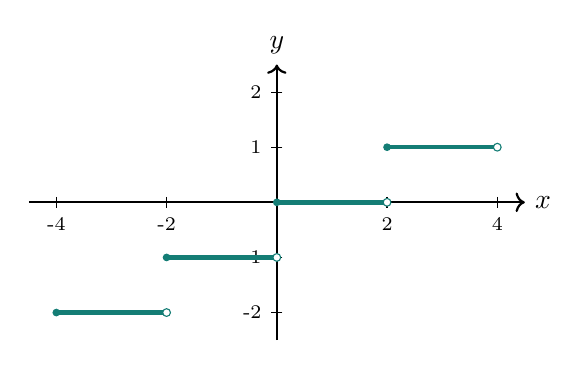
\begin{tikzpicture}[scale=0.7]
  \draw[->, thick] (-4.5,0) -- (4.5,0) node[right] {$x$};
  \draw[->, thick] (0,-2.5) -- (0,2.5) node[above] {$y$};
  \foreach \x in {-4,-2,2,4} \draw (\x,0.1) -- (\x,-0.1) node[below, font=\scriptsize] {\x};
  \foreach \y in {-2,-1,1,2} \draw (0.1,\y) -- (-0.1,\y) node[left, font=\scriptsize] {\y};
  \draw[teal, ultra thick] (-4,-2) -- (-2.05,-2);
  \fill[teal] (-4,-2) circle (2pt); \draw[teal, fill=white] (-2,-2) circle (2pt);
  \draw[teal, ultra thick] (-2,-1) -- (-0.05,-1);
  \fill[teal] (-2,-1) circle (2pt); \draw[teal, fill=white] (0,-1) circle (2pt);
  \draw[teal, ultra thick] (0,0) -- (1.95,0);
  \fill[teal] (0,0) circle (2pt); \draw[teal, fill=white] (2,0) circle (2pt);
  \draw[teal, ultra thick] (2,1) -- (3.95,1);
  \fill[teal] (2,1) circle (2pt); \draw[teal, fill=white] (4,1) circle (2pt);
\end{tikzpicture} &
% Ceiling plot
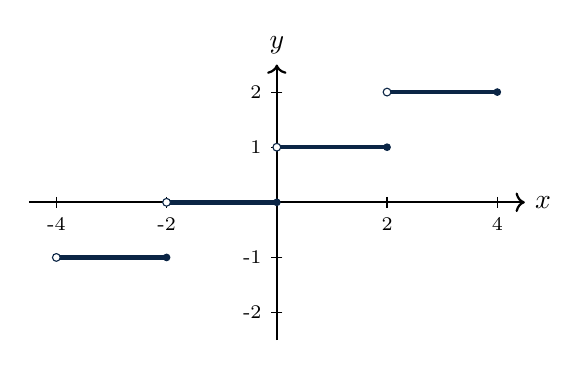
\begin{tikzpicture}[scale=0.7]
  \draw[->, thick] (-4.5,0) -- (4.5,0) node[right] {$x$};
  \draw[->, thick] (0,-2.5) -- (0,2.5) node[above] {$y$};
  \foreach \x in {-4,-2,2,4} \draw (\x,0.1) -- (\x,-0.1) node[below, font=\scriptsize] {\x};
  \foreach \y in {-2,-1,1,2} \draw (0.1,\y) -- (-0.1,\y) node[left, font=\scriptsize] {\y};
  \draw[navy, ultra thick] (-3.95,-1) -- (-2,-1);
  \draw[navy, fill=white] (-4,-1) circle (2pt); \fill[navy] (-2,-1) circle (2pt);
  \draw[navy, ultra thick] (-1.95,0) -- (0,0);
  \draw[navy, fill=white] (-2,0) circle (2pt); \fill[navy] (0,0) circle (2pt);
  \draw[navy, ultra thick] (0.05,1) -- (2,1);
  \draw[navy, fill=white] (0,1) circle (2pt); \fill[navy] (2,1) circle (2pt);
  \draw[navy, ultra thick] (2.05,2) -- (4,2);
  \draw[navy, fill=white] (2,2) circle (2pt); \fill[navy] (4,2) circle (2pt);
\end{tikzpicture} \\
\textbf{(a) } $y = \left\lfloor \frac{x}{2} \right\rfloor$ (left-closed, right-open) & \textbf{(b) } $y = \left\lceil \frac{x}{2} \right\rceil$ (left-open, right-closed)
\end{tabular}
\end{center}
\begin{itemize}
    \item For $y = \lfloor x/2 \rfloor$: On $[-4, -2)$, $y = -2$; on $[-2, 0)$, $y = -1$; on $[0, 2)$, $y = 0$; on $[2, 4)$, $y = 1$.
    \item For $y = \lceil x/2 \rceil$: On $(-4, -2]$, $y = -1$; on $(-2, 0]$, $y = 0$; on $(0, 2]$, $y = 1$; on $(2, 4]$, $y = 2$.
\end{itemize}
\end{exambox}

\begin{exambox}{[SEC Final Examination 2022, CSE 103] \ Multi-Stage Mapping Anatomy (Figure-1)}
\Qlabel
Let the functions $f\colon A\to B$, $g\colon B\to C$, and $h\colon C\to D$ be defined by Figure-1 below. Determine if each function is: (i) onto, (ii) one-to-one, (iii) invertible. \hfill\textit{[1$\times$3]}
\begin{center}
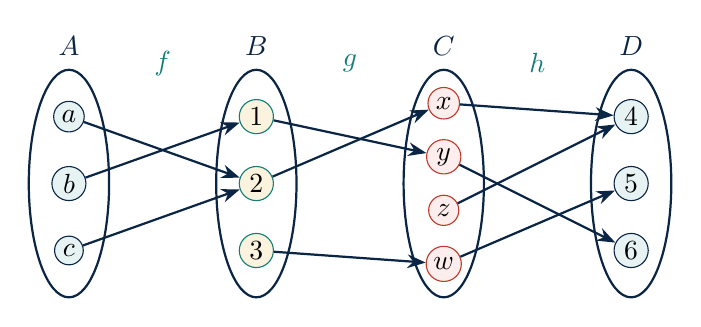
\begin{tikzpicture}[scale=0.85, >=Stealth]
  \foreach \x/\l in {0/A, 2.8/B, 5.6/C, 8.4/D} {
    \draw[navy, thick] (\x,0) ellipse (0.6 and 1.7);
    \node[font=\bfseries\color{navy}] at (\x,2.05) {$\l$};
  }
  \node[font=\bfseries\color{teal}] at (1.4,1.8) {$f$};
  \node[font=\bfseries\color{teal}] at (4.2,1.8) {$g$};
  \node[font=\bfseries\color{teal}] at (7.0,1.8) {$h$};

  \node[circle, fill=lightteal, draw=navy, inner sep=1.5pt] (Aa) at (0,1) {$a$};
  \node[circle, fill=lightteal, draw=navy, inner sep=1.5pt] (Ab) at (0,0) {$b$};
  \node[circle, fill=lightteal, draw=navy, inner sep=1.5pt] (Ac) at (0,-1) {$c$};

  \node[circle, fill=lightgold, draw=teal, inner sep=1.5pt] (B1) at (2.8,1) {$1$};
  \node[circle, fill=lightgold, draw=teal, inner sep=1.5pt] (B2) at (2.8,0) {$2$};
  \node[circle, fill=lightgold, draw=teal, inner sep=1.5pt] (B3) at (2.8,-1) {$3$};

  \node[circle, fill=lightcoral, draw=coral, inner sep=1.5pt] (Cx) at (5.6,1.2) {$x$};
  \node[circle, fill=lightcoral, draw=coral, inner sep=1.5pt] (Cy) at (5.6,0.4) {$y$};
  \node[circle, fill=lightcoral, draw=coral, inner sep=1.5pt] (Cz) at (5.6,-0.4) {$z$};
  \node[circle, fill=lightcoral, draw=coral, inner sep=1.5pt] (Cw) at (5.6,-1.2) {$w$};

  \node[circle, fill=lightteal, draw=navy, inner sep=1.5pt] (D4) at (8.4,1) {$4$};
  \node[circle, fill=lightteal, draw=navy, inner sep=1.5pt] (D5) at (8.4,0) {$5$};
  \node[circle, fill=lightteal, draw=navy, inner sep=1.5pt] (D6) at (8.4,-1) {$6$};

  \begin{scope}[->, thick, navy]
    \draw (Aa) -- (B2); \draw (Ab) -- (B1); \draw (Ac) -- (B2);
    \draw (B1) -- (Cy); \draw (B2) -- (Cx); \draw (B3) -- (Cw);
    \draw (Cx) -- (D4); \draw (Cy) -- (D6); \draw (Cz) -- (D4); \draw (Cw) -- (D5);
  \end{scope}
\end{tikzpicture}\\[2pt]
{\footnotesize\textbf{Figure-1:} Functional chains across four finite alphabets.}
\end{center}
\tcblower
\Alabel
A function is \textbf{invertible} if and only if it is a \textbf{bijection} (both one-to-one and onto):
\begin{enumerate}
    \item \textbf{Function $f\colon A\to B$:}
    \begin{itemize}
        \item \textbf{One-to-one:} \textbf{No} --- both $a$ and $c$ map to the same image: $f(a) = f(c) = 2$ ($a \neq c$).
        \item \textbf{Onto:} \textbf{No} --- element $3 \in B$ has no preimage; $\operatorname{Range}(f) = \{1, 2\} \neq B$.
        \item \textbf{Invertible:} \textbf{No} (not a bijection).
    \end{itemize}
    \item \textbf{Function $g\colon B\to C$:}
    \begin{itemize}
        \item \textbf{One-to-one:} \textbf{Yes} --- distinct inputs produce distinct outputs: $g(1)=y, g(2)=x, g(3)=w$.
        \item \textbf{Onto:} \textbf{No} --- target element $z \in C$ has no incoming edge; $\operatorname{Range}(g) = \{x, y, w\} \subsetneq C$.
        \item \textbf{Invertible:} \textbf{No} (fails surjectivity).
    \end{itemize}
    \item \textbf{Function $h\colon C\to D$:}
    \begin{itemize}
        \item \textbf{One-to-one:} \textbf{No} --- collision at output $4$: $h(x) = h(z) = 4$ ($x \neq z$).
        \item \textbf{Onto:} \textbf{Yes} --- every target element in $D=\{4,5,6\}$ has at least one preimage: $h(x)=4, h(w)=5, h(y)=6$.
        \item \textbf{Invertible:} \textbf{No} (fails injectivity).
    \end{itemize}
\end{enumerate}
\end{exambox}

\begin{exambox}{[SEC Final 2022 \& CSE 143 Final 2023] \ Floor \& Ceiling Numerical Evaluations}
\Qlabel
Evaluate the exact numerical value of each expression:
\[
\text{(a) } \lfloor 7.5\rfloor, \ \lfloor -7.5\rfloor, \ \lfloor -18\rfloor \qquad
\text{(b) } \lceil 7.5\rceil, \ \lceil -7.5\rceil, \ \lceil -18\rceil \qquad
\text{(c) } \left\lfloor\frac{1}{5}\right\rfloor, \ \lceil 2.5\rceil, \ \lfloor -2.99\rfloor, \ \left\lceil-\frac{1}{2}\right\rceil
\]
\hfill\textit{[2+2]}
\tcblower
\Alabel
Recall that $\lfloor x \rfloor$ is the largest integer $\le x$, and $\lceil x \rceil$ is the smallest integer $\ge x$:
\begin{itemize}
    \item $\lfloor 7.5 \rfloor = \mathbf{7}$, \quad $\lfloor -7.5 \rfloor = \mathbf{-8}$ \ \textit{(since $-8 < -7.5 < -7$)}, \quad $\lfloor -18 \rfloor = \mathbf{-18}$.
    \item $\lceil 7.5 \rceil = \mathbf{8}$, \quad $\lceil -7.5 \rceil = \mathbf{-7}$, \quad $\lceil -18 \rceil = \mathbf{-18}$.
    \item $\left\lfloor\frac{1}{5}\right\rfloor = \lfloor 0.2 \rfloor = \mathbf{0}$.
    \item $\lceil 2.5 \rceil = \mathbf{3}$.
    \item $\lfloor -2.99 \rfloor = \mathbf{-3}$ \ \textit{(the greatest integer $\le -2.99$ is $-3$)}.
    \item $\left\lceil-\frac{1}{2}\right\rceil = \lceil -0.5 \rceil = \mathbf{0}$.
\end{itemize}
\end{exambox}

\begin{exambox}{[SEC Final 2022 / TT-01 / Final 2024] \ The Ackermann Function: $A(1,3)$ and $A(2,2)$}
\Qlabel
The \textbf{Ackermann function} $A(m, n)$ on non-negative integers $\mathbb{N}_0 \times \mathbb{N}_0$ is defined recursively by:
\[
A(m, n) = \begin{cases}
n + 1 & \text{if } m = 0 \\
A(m - 1, 1) & \text{if } m > 0 \text{ and } n = 0 \\
A(m - 1, A(m, n - 1)) & \text{if } m > 0 \text{ and } n > 0
\end{cases}
\]
(a) State the conditions and compute $A(1, 3)$. \hfill\textit{[5]}\\
(b) Use the formal definition to evaluate $A(2, 2)$. \hfill\textit{[3]}
\tcblower
\Alabel
\textbf{(a) Step-by-step Evaluation of $A(1, 3)$:}
First, evaluate the base sequence for $m = 1$:
\begin{align*}
A(1, 0) &= A(0, 1) = 1 + 1 = \mathbf{2} \\
A(1, 1) &= A(0, A(1, 0)) = A(0, 2) = 2 + 1 = \mathbf{3} \\
A(1, 2) &= A(0, A(1, 1)) = A(0, 3) = 3 + 1 = \mathbf{4} \\
A(1, 3) &= A(0, A(1, 2)) = A(0, 4) = 4 + 1 = \mathbf{5}
\end{align*}
\textit{Closed-form law for $m=1$:} In general, $\mathbf{A(1, n) = n + 2}$. Thus, $\mathbf{A(1, 3) = 5}$.

\medskip
\textbf{(b) Step-by-step Evaluation of $A(2, 2)$:}
For $m = 2$, we apply $A(2, n) = A(1, A(2, n-1))$ and use our closed form $A(1, k) = k + 2$:
\begin{align*}
A(2, 0) &= A(1, 1) = 1 + 2 = \mathbf{3} \\
A(2, 1) &= A(1, A(2, 0)) = A(1, 3) = 3 + 2 = \mathbf{5} \\
A(2, 2) &= A(1, A(2, 1)) = A(1, 5) = 5 + 2 = \mathbf{7}
\end{align*}
\textit{Closed-form law for $m=2$:} In general, $\mathbf{A(2, n) = 2n + 3}$. Thus, $\mathbf{A(2, 2) = 7}$.
\end{exambox}

\begin{exambox}{[SEC Final Examination 2023, CSE 143] \ Bijectivity Analysis of $f(x) = x^2+1$ on $\mathbb{R}\to\mathbb{R}$}
\Qlabel
Let $f(x) = x^2 + 1$ be a function from $\mathbb{R}$ to $\mathbb{R}$. Is it a one-to-one correspondence (bijection)? Justify your answer. \hfill\textit{[4]}
\tcblower
\Alabel
A one-to-one correspondence requires the function to be simultaneously \textbf{injective} and \textbf{surjective}:
\begin{enumerate}
    \item \textbf{Injectivity (One-to-One) Test:}
    Consider $x_1 = 1$ and $x_2 = -1$:
    \[
    f(1) = 1^2 + 1 = 2, \qquad f(-1) = (-1)^2 + 1 = 2.
    \]
    Since $f(1) = f(-1)$ but $1 \neq -1$, $f$ fails the injectivity criterion. $f$ is \textbf{NOT one-to-one}.
    
    \item \textbf{Surjectivity (Onto) Test:}
    For any real number $x \in \mathbb{R}$, $x^2 \ge 0 \implies x^2 + 1 \ge 1$.
    Thus, the range of $f$ is:
    \[
    \operatorname{Range}(f) = [1, \infty) \subsetneq \mathbb{R}.
    \]
    Any target element $y < 1$ (for example, $y = 0 \in \mathbb{R}$) has no real preimage because $x^2 + 1 = 0 \implies x^2 = -1$ has no solution in $\mathbb{R}$. Thus, $f$ is \textbf{NOT onto}.
\end{enumerate}
\textbf{Conclusion:} Because $f$ fails both injectivity and surjectivity, it is \textbf{NOT a one-to-one correspondence}.
\end{exambox}

\begin{exambox}{[SEC Final Examination 2023, CSE 143] \ Integer Function Compositions}
\Qlabel
Let $f$ and $g$ be functions from $\mathbb{Z}$ to $\mathbb{Z}$ defined by $f(x) = 2x + 3$ and $g(x) = 3x^2 + 2$. Determine $f \circ g(3)$ and $g \circ f(1)$. \hfill\textit{[4]}
\tcblower
\Alabel
By definition of function composition, $(f \circ g)(x) = f(g(x))$ and $(g \circ f)(x) = g(f(x))$:
\begin{enumerate}
    \item \textbf{Compute $f \circ g(3)$:}
    First evaluate the inner function at $x = 3$:
    \[
    g(3) = 3(3^2) + 2 = 3(9) + 2 = 27 + 2 = 29
    \]
    Now evaluate the outer function at $29$:
    \[
    f(g(3)) = f(29) = 2(29) + 3 = 58 + 3 = \mathbf{61}.
    \]
    \item \textbf{Compute $g \circ f(1)$:}
    First evaluate the inner function at $x = 1$:
    \[
    f(1) = 2(1) + 3 = 2 + 3 = 5
    \]
    Now evaluate the outer function at $5$:
    \[
    g(f(1)) = g(5) = 3(5^2) + 2 = 3(25) + 2 = 75 + 2 = \mathbf{77}.
    \]
\end{enumerate}
Observe that $f \circ g \neq g \circ f$, verifying that function composition is non-commutative.
\end{exambox}

\begin{exambox}{[SEC Final Examination, CSE 0541 1143] \ Natural Number Mapping: $f(x) = 2x+1$ on $\mathbb{N}\to\mathbb{N}$}
\Qlabel
A function $f\colon \mathbb{N} \to \mathbb{N}$ is defined as $f(x) = 2x + 1$ (where $\mathbb{N} = \{1, 2, 3, \dots\}$). Determine if $f$ is one-to-one and onto. Justify your answer. \hfill\textit{[03]}
\tcblower
\Alabel
\begin{enumerate}
    \item \textbf{One-to-One (Injective):}
    Let $a, b \in \mathbb{N}$ such that $f(a) = f(b)$:
    \[
    2a + 1 = 2b + 1 \implies 2a = 2b \implies a = b.
    \]
    Since $f(a) = f(b)$ implies $a = b$ for all $a, b \in \mathbb{N}$, $f$ is strictly \textbf{one-to-one (injective)}.
    
    \item \textbf{Onto (Surjective):}
    For $f$ to be onto, every $y \in \mathbb{N}$ must have a preimage $x \in \mathbb{N}$ satisfying $2x + 1 = y \implies x = \frac{y - 1}{2}$.
    \begin{itemize}
        \item For $y = 2 \in \mathbb{N}$ (or any even number): $x = \frac{2 - 1}{2} = \frac{1}{2} \notin \mathbb{N}$.
        \item The range of $f$ consists only of odd natural numbers: $\operatorname{Range}(f) = \{3, 5, 7, \dots\} \neq \mathbb{N}$.
    \end{itemize}
    Since even natural numbers have no integer preimages in $\mathbb{N}$, $f$ is \textbf{NOT onto (not surjective)}.
\end{enumerate}
\end{exambox}

\begin{exambox}{[SEC Final Examination 2024, CSE 0541 1143] \ Triple Function Compositions on $X = \{1, 2, 3\}$}
\Qlabel
Let $f, g, h$ be functions on $X = \{1, 2, 3\}$ defined as:
\[
f = \{(1, 2), (2, 3), (3, 1)\}, \quad g = \{(1, 2), (2, 1), (3, 3)\}, \quad h = \{(1, 1), (2, 2), (3, 1)\}
\]
Compute: \ (i) $f \circ g \circ h$ \qquad (ii) $f \circ h \circ g$. \hfill\textit{[04]}
\tcblower
\Alabel
Recall that $(f \circ g \circ h)(x) = f(g(h(x)))$ evaluates from \textbf{right to left}:
\begin{enumerate}
    \item \textbf{(i) Compute $f \circ g \circ h$:}
    \begin{itemize}
        \item For $x = 1$: $h(1) = 1 \implies g(1) = 2 \implies f(2) = 3 \implies (1, 3)$.
        \item For $x = 2$: $h(2) = 2 \implies g(2) = 1 \implies f(1) = 2 \implies (2, 2)$.
        \item For $x = 3$: $h(3) = 1 \implies g(1) = 2 \implies f(2) = 3 \implies (3, 3)$.
    \end{itemize}
    \[
    \mathbf{f \circ g \circ h = \big\{ (1, 3), \, (2, 2), \, (3, 3) \big\}}
    \]
    
    \item \textbf{(ii) Compute $f \circ h \circ g$:}
    \begin{itemize}
        \item For $x = 1$: $g(1) = 2 \implies h(2) = 2 \implies f(2) = 3 \implies (1, 3)$.
        \item For $x = 2$: $g(2) = 1 \implies h(1) = 1 \implies f(1) = 2 \implies (2, 2)$.
        \item For $x = 3$: $g(3) = 3 \implies h(3) = 1 \implies f(1) = 2 \implies (3, 2)$.
    \end{itemize}
    \[
    \mathbf{f \circ h \circ g = \big\{ (1, 3), \, (2, 2), \, (3, 2) \big\}}
    \]
\end{enumerate}
\end{exambox}

\begin{exambox}{[SEC TT-02 / Final Examination 2024] \ Non-Linear Recursive Sequence}
\Qlabel
Find $f(4)$ if $f$ is defined recursively on integers by:
\[
f(0) = -1, \quad f(1) = 2, \quad \text{and} \quad f(n + 1) = f(n)^2 \cdot f(n - 1) \quad \text{for } n \ge 1.
\]
\hfill\textit{[02 / 03]}
\tcblower
\Alabel
We compute subsequent terms iteratively using the recursive relation:
\begin{enumerate}
    \item For $n = 1$:
    \[
    f(2) = f(1)^2 \cdot f(0) = (2)^2 \cdot (-1) = 4 \cdot (-1) = \mathbf{-4}.
    \]
    \item For $n = 2$:
    \[
    f(3) = f(2)^2 \cdot f(1) = (-4)^2 \cdot (2) = 16 \cdot 2 = \mathbf{32}.
    \]
    \item For $n = 3$:
    \[
    f(4) = f(3)^2 \cdot f(2) = (32)^2 \cdot (-4) = 1024 \cdot (-4) = \mathbf{-4096}.
    \]
\end{enumerate}
Therefore, $\mathbf{f(4) = -4096}$.
\end{exambox}

% ==============================================================================
% MODULE 9: SUMMARY
% ==============================================================================
\newpage
\section{Summary}

\subsection{Fundamental Definitions, Axioms \& Inclusion Statements}
\begin{defbox}[Core Axiomatic Statements \& Definitions]
\begin{itemize}
    \item \textbf{Set Membership vs. Inclusion:}
    \[
    x \in A \quad \text{(element belongs to set)} \qquad \text{vs.} \qquad A \subseteq B \iff (\forall x)(x \in A \implies x \in B)
    \]
    \item \textbf{\color{gold!90!black}$\bigstar$ Set Equality Principle (Double Inclusion):}
    \[
    A = B \iff (A \subseteq B \ \land \ B \subseteq A) \iff (\forall x)(x \in A \iff x \in B)
    \]
    \item \textbf{\color{gold!90!black}$\bigstar$ The Empty Set ($\emptyset$) Axioms:}
    \[
    \emptyset = \{\}, \qquad |\emptyset| = 0, \qquad \emptyset \subseteq A \quad (\forall A), \qquad \emptyset \in \mathcal{P}(A) \quad (\forall A)
    \]
    \item \textbf{Proper Subset Criterion:}
    \[
    A \subset B \iff (A \subseteq B \ \land \ A \neq B)
    \]
    \item \textbf{Universal Set Bounds:}
    \[
    \forall A \subseteq \mathcal{U}: \quad \emptyset \subseteq A \subseteq \mathcal{U}, \qquad \overline{\mathcal{U}} = \emptyset, \qquad \overline{\emptyset} = \mathcal{U}
    \]
    \item \textbf{\color{gold!90!black}$\bigstar$ Fundamental Set Operations \& Subsumption Equivalences:}
    \[
    A \subseteq B \iff A \cap B = A \iff A \cup B = B \iff A \setminus B = \emptyset \iff \overline{B} \subseteq \overline{A}
    \]
    \item \textbf{\color{gold!90!black}$\bigstar$ Binary Relations, Domain \& Range:} For any relation $R \subseteq A \times B$:
    \[
    \text{Dom}(R) = \{a \in A \mid \exists b \in B, \, (a, b) \in R\}, \qquad \text{Range}(R) = \{b \in B \mid \exists a \in A, \, (a, b) \in R\}
    \]
    \item \textbf{\color{gold!90!black}$\bigstar$ Reflexive Relation Criterion:}
    \[
    \forall a \in A, \, (a, a) \in R \iff \text{All diagonal entries } m_{ii} = 1 \iff \text{Self-loops on all digraph vertices}
    \]
    \item \textbf{\color{gold!90!black}$\bigstar$ Function Single-Valuedness Axiom:}
    \[
    f: A \to B \iff \forall a \in A, \ \exists! b \in B, \ (a, b) \in f \qquad \text{with } \operatorname{Range}(f) \subseteq \operatorname{Codom}(f)
    \]
    \item \textbf{\color{gold!90!black}$\bigstar$ Invertibility Principle:}
    \[
    f^{-1}: B \to A \text{ exists} \iff f \text{ is Bijective (Injective } \land \text{ Surjective)}
    \]
    \item \textbf{\color{gold!90!black}$\bigstar$ Composition Law \& Identity:}
    \[
    (f \circ g)(x) = f(g(x)), \qquad f \circ f^{-1} = \operatorname{id}_B, \qquad f^{-1} \circ f = \operatorname{id}_A
    \]
    \item \textbf{Floor \& Ceiling Bound Axiom:}
    \[
    x - 1 < \lfloor x \rfloor \le x \le \lceil x \rceil < x + 1, \qquad \lfloor x + n \rfloor = \lfloor x \rfloor + n \quad (\forall n \in \mathbb{Z})
    \]
\end{itemize}
\end{defbox}

\newpage
\subsection{Cardinality, Enumeration \& Combinatorial Formulae}
\begin{notebox}[Essential Counting Formulae Compendium]
\renewcommand{\arraystretch}{1.15}
\begin{tabularx}{\linewidth}{@{}l X l@{}}
\toprule
\textbf{\color{navy}Concept} & \textbf{\color{navy}Formula} & \textbf{\color{navy}Condition / Context} \\
\midrule
\textbf{\color{gold!90!black}$\bigstar$ Set Cardinality} & $|A| = n$ & Number of distinct elements in $A$ \\
\textbf{\color{gold!90!black}$\bigstar$ Power Set Cardinality} & $|\mathcal{P}(A)| = 2^{|A|} = 2^n$ & Any finite set of size $n$ \\
\textbf{\color{gold!90!black}$\bigstar$ Total Subsets} & $N_{\text{total}} = 2^n$ & Includes $\emptyset$ and $A$ \\
\textbf{Proper Subsets} & $N_{\text{proper}} = 2^n - 1$ & Excludes $A$ itself \\
\textbf{Non-Empty Subsets} & $N_{\text{non-empty}} = 2^n - 1$ & Excludes $\emptyset$ \\
\textbf{Non-Empty Proper Subsets} & $N_{\text{ne-proper}} = 2^n - 2$ & Excludes both $\emptyset$ and $A$ \\
\textbf{Cartesian Product Size} & $|A \times B| = |A| \cdot |B|$ & Ordered pairs: $(a, b) \neq (b, a)$ \\
\textbf{General Cartesian Size} & $|A_1 \times \dots \times A_k| = \prod_{i=1}^k |A_i|$ & $k$-ary Cartesian product \\
\textbf{Total Binary Relations} & $|\mathcal{P}(A \times B)| = 2^{|A| \cdot |B|}$ & Number of binary relations \\
\textbf{\color{gold!90!black}$\bigstar$ Reflexive Relations Count} & $N_{\text{reflexive}} = 2^{n(n-1)}$ & Distinct reflexive relations on size $n$ \\
\textbf{\color{gold!90!black}$\bigstar$ Total Functions $A \to B$} & $N_{\text{functions}} = |B|^{|A|}$ & Unrestricted mappings \\
\textbf{\color{gold!90!black}$\bigstar$ Total Injections (One-to-One)} & $P(|B|, |A|) = \frac{|B|!}{(|B|-|A|)!}$ & Requires $|A| \le |B|$ \\
\textbf{\color{gold!90!black}$\bigstar$ Total Bijections (Correspondences)} & $N_{\text{bijections}} = n!$ & Finite sets with $|A| = |B| = n$ \\
\textbf{\color{gold!90!black}$\bigstar$ Difference Cardinality} & $|A \setminus B| = |A| - |A \cap B|$ & Relative complement size \\
\textbf{\color{gold!90!black}$\bigstar$ Symmetric Diff. Size} & $|A \oplus B| = |A \cup B| - |A \cap B|$ & Elements in exactly one set \\
\textbf{\color{gold!90!black}$\bigstar$ Complement Cardinality} & $|\overline{A}| = |\mathcal{U}| - |A|$ & Unshaded universe region \\
\textbf{PIE (2 Sets)} & $|A \cup B| = |A| + |B| - |A \cap B|$ & Subtracts overlap once \\
\textbf{PIE (3 Sets)} & $|A \cup B \cup C| = \sum |A_i| - \sum |A_i \cap A_j| + |A \cap B \cap C|$ & Full 3-set inclusion-exclusion \\
\textbf{Binary Representation Bits} & $b(n) = \lfloor \log_2 n \rfloor + 1$ & Bits to store integer $n > 0$ \\
\bottomrule
\end{tabularx}
\end{notebox}

\vspace{-4pt}
\subsection{Set Identities and Algebraic Laws}
\begin{examplebox}[Set Identities and Algebraic Laws]
\renewcommand{\arraystretch}{1.12}
\begin{tabularx}{\linewidth}{@{}l X X@{}}
\toprule
\textbf{\color{navy}Law Name} & \textbf{\color{teal}Union Form ($\cup$)} & \textbf{\color{teal}Intersection Form ($\cap$)} \\
\midrule
\textbf{\color{gold!90!black}$\bigstar$ Identity Laws} & $A \cup \emptyset = A$ & $A \cap \mathcal{U} = A$ \\
\textbf{\color{gold!90!black}$\bigstar$ Domination Laws} & $A \cup \mathcal{U} = \mathcal{U}$ & $A \cap \emptyset = \emptyset$ \\
\textbf{\color{gold!90!black}$\bigstar$ Idempotent Laws} & $A \cup A = A$ & $A \cap A = A$ \\
\textbf{\color{gold!90!black}$\bigstar$ Double Complement} & \multicolumn{2}{c}{$\overline{\overline{A}} = A$ \quad (Involution Law)} \\
\textbf{\color{gold!90!black}$\bigstar$ Commutative Laws} & $A \cup B = B \cup A$ & $A \cap B = B \cap A$ \\
\textbf{\color{gold!90!black}$\bigstar$ Associative Laws} & $(A \cup B) \cup C = A \cup (B \cup C)$ & $(A \cap B) \cap C = A \cap (B \cap C)$ \\
\textbf{\color{gold!90!black}$\bigstar$ Distributive Laws} & $A \cup (B \cap C) = (A \cup B) \cap (A \cup C)$ & $A \cap (B \cup C) = (A \cap B) \cup (A \cap C)$ \\
\textbf{\color{gold!90!black}$\bigstar$ De Morgan's Laws} & $\overline{A \cup B} = \overline{A} \cap \overline{B}$ & $\overline{A \cap B} = \overline{A} \cup \overline{B}$ \\
\textbf{\color{gold!90!black}$\bigstar$ Absorption Laws} & $A \cup (A \cap B) = A$ & $A \cap (A \cup B) = A$ \\
\textbf{\color{gold!90!black}$\bigstar$ Complement Laws} & $A \cup \overline{A} = \mathcal{U}$ & $A \cap \overline{A} = \emptyset$ \\
\textbf{\color{gold!90!black}$\bigstar$ Difference Law} & \multicolumn{2}{c}{$A \setminus B = A \cap \overline{B}$} \\
\textbf{\color{gold!90!black}$\bigstar$ Symmetric Difference} & \multicolumn{2}{c}{$A \oplus B = (A \setminus B) \cup (B \setminus A) = (A \cup B) \setminus (A \cap B)$} \\
\bottomrule
\end{tabularx}
\end{examplebox}

\vspace{6pt}
\begin{center}
{\small\color{navy}\textbf{--- END OF SETS, RELATIONS \& FUNCTIONS ---}}
\end{center}

\end{document}
